% This is a template for use with the MSU Thesis class
%
% Class options: 
% PhD for dissertations;
% MA for Master of Arts 
% MS for Master of Science
% MAT for Master of Arts for Teachers  
% MBA for Master of Business Administration  
% MFA for Master of Fine Arts  
% MIPS for Master of International Planning Studies  
% MHRL for Master of Human Resources and Labor Relations  
% MMus for Master of Music  
% MSN for Master of Science in Nursing  
% MPP for Master of Public Policy  
% MSW for Master of Social Work  
% MURP for Master in Urban and Regional Planning  
%
% Default is PhD
%
%
% This template has everything in the right order.
% Just add real content and you're done!
%
\documentclass[lscape]{msu-thesis}
%
% for a prettier, but possibly non-compliant table of contents use the [mixedtoc] option
% for a plain table of contents use the [plaintoc] option
% for a horrendous looking, but possibly required table of contents, use the [boldtoc] option
%
% If you have large tables/figures that need to be in landscape mode, add the [lscape] option

% This is standard fontenc/inputenc for pdflatex
% If you use LuaLaTeX or XeLaTeX you should replace this with the fontspec package
\usepackage[utf8]{inputenc}
\usepackage[T1]{fontenc}
\usepackage{graphicx}
%
% If the thesis office requires Times, we'll give them Times
% You can experiment with other font packages here if you like.
% If you are using XeLaTeX or LuaLaTeX load the Times or Times New Roman font with \setmainfont
\usepackage{mathptmx} 
\graphicspath{{images/}}
%
% Load any extra packages here
%
% You must specify the title of your thesis, your name, the field of study (not department), and the year
\title{Identification of candidate genes and isoforms associated with
genetic resistance to Marek's Disease from RNA-Seq data}
\author{Likit Preeyanon}
\fieldofstudy{Microbiology and Molecular Genetics} % This should be in sentence case
\date{2014}

% If you want a dedication page, specify the text of the dedication here and uncomment the next command.
%
\dedication{To scientists who encourage open science.}
%
\begin{document}

% All the stuff before your actual chapters is called the front matter
\frontmatter
% First make the title page
\maketitlepage
% Next make the abstract
\begin{abstract}

Marek's disease (MD) in chickens is characterized by T cell
lymphomas caused by the Marek's disease virus (MDV), an
$\alpha$-herpesvirus. MD is a major economical problem for
the poultry industry as it causes approximately \$2 billion
in worldwide losses annually. Although vaccination has been
effective at preventing tumor formation, it has not been
able to prevent MDV infection or replication.  Consequently,
more virulent field strains have emerged over the past
decades following the introduction of new vaccines. Poor
practices of vaccination and incomplete immunity have been
speculated to play a role in driving the evolution of the
virus with greater virulence. Therefore, it is critically
important to develop more sustainable control measures to
the disease in the long run.

Development of genetically resistant chickens has been an
alternative approach to control the virus and a number of studies
have been conducted to identify specific genes that contribute to
MD resistance. The major histocompatibility (MHC) locus has been
found to be strongly associated with resistance or susceptibility
to MD, and several alleles have been well characterized.  Non-MHC
genes also play a major role in resistance to MD. Two inbred
lines (line 6 and line 7) maintained at Avian and Oncology
Laboratory share the same MHC allele (B\textsuperscript{2}), yet
line 6 is resistant and line 7 is susceptible to MD,
respectively.  These two lines have been used as a model to study
non-MHC genes that contribute to resistance and susceptibility to
the disease.

To identify non-MHC genes contributing resistance to MD, a
computational pipeline was developed to integrate gene models
from Ensembl, {\em de novo} assembly, and reference-based
assembly (Cufflinks) of sequencing reads to construct a more
complete set of gene models that include more complete
untranslated regions (UTRs) and isoforms predicted from RNA-Seq
data. The results from expression analysis suggest that the
immune response in line 7 is more active at the early stage of
infection (4 days post-infection) compared to line 6.
Differentially expressed genes are enriched in pathways involved
in both the innate and the adaptive immune response in line 7,
whereas, only genes involved in the innate immune response are
significantly enriched in line 6. Due to the cell-associated
nature of MDV and the current model of MDV infection, the virus
is thought to transfer from B cells and antigen presenting cells
(APCs) to activated T cells during the lytic infection.
Therefore, repressed or delayed activation of the adaptive immune
response in line 6 may be a key mechanism conferring MD
resistance.

Investigation of differential exon usage suggests that genes
involved in the cytoskeleton pathway may play a role in
repressing the activation of the adaptive immune response.
For instance, the {\em ITGB2} gene encodes integrin $\beta$2, a component
of several molecules including the lymphocyte
function-associated antigen 1 (LFA-1). LFA-1 is exclusively
expressed on the surface of leukocytes and plays an
important role in cell-to-cell contact and antigen
presentation.  It could be speculated that an alternative
isoform of {\em ITGB2} affects a function of LFA-1 and prevents T
cells from being activated by APCs or B cells resulting in
the delayed activation of the adaptive immune response or
the lower number of activated T cells, the target of MDV.

The results from this study show that many genes not identified
as differentially expressed at a gene level are differentially
expressed at an isoform level; therefore, they will not be
identified by gene expression analysis alone. Using the pipeline
developed in this study, one can iteratively incorporate ENSEMBL
models and RNA-seq data to construct better gene models that
include genes and isoforms expressed in all samples and perform
differential gene and isoform expression analysis to identify
genes and isoforms that are responsible for resistance to MD.

Although functions of most isoforms are not fully annotated,
we have shown that methods, such as protein prediction and
pathway analysis, can be used to predict the putative
functions of the isoforms and their potential roles in MD
resistance, which could open up a new direction for MD
research. Moreover, prediction of causative {\em cis}-regulatory
elements in those genes will lead to identification of
precise genetic factors contributing to MD resistance.

\end{abstract}

% Force a newpage
\clearpage
% Make the copyright page. The Graduate School ridiculously prohibits you
% from having a copyright page unless you pay ProQuest to register the copyright.
% This should be illegal, but I didn't make up the rule.

% \makecopyrightpage

% If you have a dedication page, uncomment the next command to print the dedication page
\makededicationpage
%
\clearpage
% Your Acknowledgements are formatted like a chapter, but with no number
\chapter*{Acknowledgements}
\DoubleSpacing % Acknowledgements should be double spaced
I would like to express my special appreciation and thanks
to my mentor, Dr. C. Titus Brown, for your guidance on how
to be a good scientist and how to lead an awesome life. You
have positively influenced me both inside and outside
academia and your advice on both research and career have
been invaluable. I would also like to thank my current and
emeritus committees, Dr.  Hans H.  Cheng, Dr.  Wenjiang Fu,
Dr.  Jerry Dodgson, Dr.  Kefei Yu, Dr.  Ian York, and Dr.
Walter J. Esselman for serving as my guidance committee even
at hardship. I also thank for your brilliant comments and
suggestions. I would also like to thank Institute for
Cyber-Enabled Research (iCER) at MSU for a superb service
that enabled my research work. I also want to thank all
members of Genomics, Evolution, and Development (GED) lab
and Dr. Cheng's lab at Avian Disease and Oncology Laboratory
(ADOL), and all my collaborators for providing a friendly
working environment, friendship and all research support.

Last but not least, I would like to thank the Royal Thai
government for a five-year financial support and staff at
The Office Of Educational Affairs (OEADC) for all help and
support during my graduate study.

\clearpage
% We need to turn single spacing back on for the contents/figures/tables lists
\SingleSpacing
\tableofcontents* % table of contents will not be listed in the TOC
\clearpage
\listoftables % comment this out if you have no tables
\clearpage
\listoffigures % comment this out if you have no figures
%
% If you have a list of abbreviations/symbols it would go here preceded by a \clearpage
%
\mainmatter
%
% The next line removes the dots in chapter headings in the TOC
% May violate thesis office rules
%\addtocontents{toc}{\protect\renewcommand{\protect\cftchapterdotsep} {\cftnodots}}

\chapter{Introduction}
\section{Overview}

Marek's disease (MD) is a lymphoproliferative disease of chickens
caused by a highly oncogenic Marek's disease virus (MDV).
Vaccination has been effective in reducing tumor formation and
loss from MD; however, it does not confer protective immunity
against infection and shedding of MDV~\cite{gimeno2008marek}.
Continuous shedding of viruses from feather follicles of
vaccinated chickens allows field viruses to circulate in the
flock~\cite{morrow2004marek}.  As a consequence, more virulent
strains that overcome vaccinal protection have
emerged~\cite{witter1998control,gimeno2008marek} leading to
outbreaks that have cost an estimate of \$2
billion~\cite{morrow2004marek}.  Selective breeding of resistant
birds is an alternative control measure against MD.  In this
study, we use transcriptome data from next-generation sequencing
to compare gene and isoform expression in response to MDV
infection between MD resistant (line 6) and susceptible (line 7)
chickens in order to identify candidate genes and isoforms that
contribute to resistance to MD.

\section{Background}
\subsection{Genetic resistance to MD}

Genetic resistance to MD can be categorized into {\em MHC}
and {\em non-MHC} associated forms.  The {\em MHC} locus (B
system haplotypes) is strongly associated with MD resistance
and the phenotypes of different haplotypes have been well
characterized.  For example, B\textsuperscript{21},
B\textsuperscript{2} and B\textsuperscript{6} alleles are
usually associated with MD resistance, on the other hand,
B\textsuperscript{5}, B\textsuperscript{13} and
B\textsuperscript{19} are associated with susceptibility.
Chickens with homozygous B\textsuperscript{21} were most
resistant to MD ($0\%$), whereas, chicken heterozygous with
other alleles and B\textsuperscript{21} developed $40-93\%$
MD~\cite{briles1980identification}.  However, in some
populations, the association of B haplotypes does not follow
the aforementioned patterns. For example, the Cornell
chicken strains C and K were selected for resistance to MD,
yet strain C possesses B\textsuperscript{6},
B\textsuperscript{13} and B\textsuperscript{15} and strain K
possesses
B\textsuperscript{15}~\cite{bacon1987influence,briles1980identification}.
Similarly, inbred chicken lines 6 and 7 selected for
resistance and susceptible to MD are both
B\textsuperscript{2,2} homozygous.  This suggests that genes
outside the {\em MHC} locus also contribute to MD
resistance.

It has been postulated that different mechanisms are
controlled by {\em MHC} and {\em non-MHC}
loci~\cite{kaiser2003differential}.  For instance, Kaiser et
al.~\cite{kaiser2003differential} reported that the level of
MDV viral load also differed between lines 6 and N after 10
and 14 days post infection (dpi) -- the onset of latency --
and decreased to the same level by 21 dpi.  Although both
lines 6 and N are resistant to MD, the level of MDV viral
load in line 6 was significantly higher than in line N at 10
and 14 dpi (P$<0.05$).  Resistance line N is associated
with the B\textsuperscript{21} haplotype, whereas, the
resistance of line 6 is associated with the MDV1 locus.

% {\em non-MHC} genes are thought to have effects in cellular interaction,
% cytokines or innate immunity.
% {\em In vitro} and {\em in vivo} studies have shown that T cells from line 7
% absorbed a greater number of MDV and were more active to mitogen than those from
% line 6~\cite{lee1983ontogeny,powell1982mechanism}.
% It has been postulated that the resistance is attributable to an inherent
% mechanism that limits the susceptibility and the number of target T cells.

\subsection{Genome-wide scan for genes conferring resistance to MD}

Identification of precise genes is essential for developing
resistant breeds using a marker-assisted selection (MAS)
.  A genetic-driven method has been used to identify
quantitative trait loci (QTL) associated with MD resistance
or MD infection using lines 6 and 7 as parents.  Seven
significant and seven suggestive QTLs were identified by
Vallejo ~\cite{vallejo1998genetic} and
Yonash~\cite{yonash1999high}; whereas,
Bumstead~\cite{bumstead1998genomic} identified a significant
locus on chromosome 1, which is referred to as MDV1.  MDV1
region has a strong association with resistance in terms of
reduced viral level and tumour incidence.  Based on
comparative mapping analysis, this locus has shared
synteny with the mouse region that includes the {\em CMV1} and {\em
Ly49} genes.  {\em CMV1} controls resistance to murine
cytomegalovirus by affecting viral proliferaton and {\em
Ly49} serves as an inhibitor of cell killing by NK cells.
Correlation between functions of {\em CMV1} and {\em Ly49}
and resistance associated to this region is notable.

The drawback of QTL analysis of complex traits is it
requires a large population size ($>500$) to achieve
reliable results.  Ideally, a population size of $>1000$ is
needed for fine-mapping suitable for successful MAS ($<1$
cM)~\cite{young1999cautiously}.  Furthermore, only a few true
QTL of major effect can be detected in any given study
~\cite{collard2005introduction}.  Therefore, an alternative
approach that could facilitate the identification of precise
genes at a genome-wide scale is warranted.

Differential gene expression is thought to contribute to
phenotypic variation and difference in gene expression can
be controlled by genetic factors~\cite{morley2004genetic}.
Furthermore, functional analysis of differential-expressed
(DE) genes can provide an insight into pathways and
biological mechanisms that control phenotypes.  Data from
RNA-Seq can also be used to investigate mutations such as
SNPs and indels that might be responsible for phenotypic
differences.

Recently, high-throughput technologies including microarray
and next-generation sequencing (NGS) have been used to
compare gene or EST expression between MDV-infected birds of
selected resistant and susceptible lines to identify
candidate genes that contribute to MD resistance.
% need to add more about this?
Sarson~\cite{sarson2008transcriptional} used a low-density
immune-specific cDNA microarray to compare expression of
immune genes from splenocytes between resistant and
susceptible chickens, with B\textsuperscript{21} and the
B\textsuperscript{19} haplotype respectively, and found that
the percentage of differential-expressed genes between
B\textsuperscript{19} control and infected birds was
highest.  Furthermore, B cell surface markers such as {\em
Bu-1} and {\em IgM} levels were downregulated, which might
contribute to the decrease in B cells in the lytic phase of
infection.   Morgan et al~\cite{morgan2001induction} also used a DNA
microarray designed for chicken to compare the differential
expression between lines 6 and 7 at multiple time points.
Of $\sim1200$ genes and ESTs, a few genes including growth
hormone ({\em GH1}) and lymphotactin ({\em SCYC1}) were
found to be differentially expressed ($>2$ fold) and located
near the QTL region on chromosome 1 (MDV1) identified by
Bumstead~\cite{bumstead1998genomic}.  Growth hormone binds
to MDV {\em SORF2} and is associated with MD
resistance~\cite{liu2001growth} and lymphotactin serves as a
chemoattractant of CD4+ and CD8+ T cells.

The findings from these studies are interesting, yet very
limited due to the small scale of the analysis.  A
genome-wide scale microarray study was, therefore, conducted
by Smith et al~\cite{smith2011systems} to compare gene expression
between virus-infected lines 6 and 7 from spleen and thymus
at a larger scale.  In control groups, 395 genes in spleen
and 177 genes in thymus were differentially expressed
between lines 6 and 7.  Genes highly expressed in line 6 and
involved in innate immune responses include {\em DNAJC3,
DDT, NMU, GSTO1, VIP, HPS5, MMP7, FGFR3, HSCB, E2F4, SFTPA2}
and {\em GNG12}.  In infected groups, 593 genes in spleen
and 156 genes in thymus were differentially expressed
including {\em IgG-H, AMIGO2, MMP13}, and {\em CLEC3B} that
were highly expressed in line 6 and {\em AVD, IRG1, HSP25,
ART1, IL-18, NOS2A, CXCL13, CCLi2, MX1, SOCS1}, and {\em
IL-6} that were highly expressed in line 7.  Approximately
$26-30\%$ of DE genes were located in the previously reported QTL
regions, which could be potential candidate genes.

To conclude, high-throughput technologies together with
genetic approaches have been successfully used to identify
many candidate genes associated with MD resistance, which
confirms the complex nature of MD genetic resistance.
However, the interaction of these candidate genes and their
roles in disease resistance have not been fully defined.
Furthermore, only global gene expression has been used for
identification of genes conferring MD resistance, whereas,
alternative isoforms have been shown to play a significant
role in immune responses and contribute to disease
susceptibility~\cite{lynch2004consequences,wang2007splicing}.
This dissertation aims to identify both candidate genes and
isoforms that are involved in resistance to MD.

\section{Problem Statement}

In the immune system, many genes can express different
isoforms with a distinctive, synergistic or even opposing
function~\cite{lynch2004consequences,wang2007splicing}.
Expression of isoforms is regulated in part by {\em
cis-}regulatory sequences within an exon or intron of a
pre-mRNA~\cite{blencowe2000exonic}.  Although expressions of
various genes have been examined across stages of infection
and various genetic
background~\cite{smith2011systems,sarson2008transcriptional,kaiser2003differential,morgan2001induction},
the investigation of genome-wide isoform expression has not
been conducted.  The gap in the knowledge is, therefore, the
identification of candidate isoforms that contribute to MD
resistance.

Many tools are currently available for estimating gene and
isoform expression from RNA-Seq data as well as comparing
their expressions between samples (reviewed in
~\cite{trapnell2012differential}).  However, they are all
reliant on completeness of provided gene models.  Available
gene models such as Ensembl annotation do not include all
genes and isoforms; therefore, they are not ideal for
identification of candidate genes and isoforms.  In
addition, some annotated gene models do not included
unstranslated regions (UTRs) that can have important
biological functions as well as significant sizes.  Methods
for expression estimation typically infer gene expression
from the number of reads mapped to transcripts or gene
models.  Without complete gene models, the expression will
be inaccurately estimated resulting in errors in
differential expression (DE) prediction.  Consequently,
biological pathway prediction will be affected because the
prediction is based solely on results from DE prediction.

\section{Significance of Research}

The study will create a pipeline to integrate RNA-Seq data
with existing gene models to extend the models so that they
include genes, isoforms, and UTRs expressed in a sample.
The extended genes models will allow a better estimate of
genes and isoforms expression, which will be used to predict
biological pathways perturbed in responses to MDV infection.
Comparison of perturbed biological pathways between
resistant and susceptible birds will provide an insight into
genes and mechanisms that contribute to MD resistance.
Additionally, in depth investigation of isoform expression
could lead to identification of exonic SNPs that regulate
alternative splicing patterns, which could reveal
unprecedented level of molecular and genetic mechanisms that
impart resistance to MD.

\section{Outline of Dissertation}

In the first chapter, we describe a method developed to
construct gene models from different sources including {\em
de novo} assembly of short reads from RNA-Seq data, a
reference-guided assembly (Cufflinks) and Ensembl gene
models. We show that our method can be used to combine gene
models from different sources to build gene models that
include more splice variants. We also describe a local
assembly method that can enhance sensitivity of splice
variant detection. In the second chapter, we compare
results of gene expression and KEGG pathway analysis from
different gene models. We demonstrate that different gene
models give different results from pathway enrichment
analysis. In addition, we discuss the use of combined
annotation from chicken and mouse to increase sensitivity of
pathway prediction. In the last chapter, we report
differentially expressed genes and isoforms and discuss a
potential role of differentially expressed isoforms in MD
resistance.

\chapter{RNA-Seq assembly discovers many splice variants}
\section{Introduction}

Until recently, studies of alternative splicing have been limited to a
small number of genes and isoforms due to high-cost and low-throughput
sequencing of expressed sequence tags (ESTs) and full-length cDNA
libraries.  RNA sequencing (RNA-Seq) using deep short-read sequencing
has been used successfully in many studies to gain unprecedented
insight into a complexity of transcriptomes.

It has been estimated that, in human, $92-94$\% of multiexon genes
undergo alternative splicing and different isoforms are expressed in
different tissues~\cite{Wang:2008ea}.  This suggests that even in human
a large number of splice variants have not been explored.

%Since sequences from RNA-Seq (reads) are very short (~50--250bp for Illumina
%reads), it is not feasible to assess expression isoforms and their structures
%without mapping reads to a reference annotation or reconstructing a full-length
%transcript from short reads.

Despite the small size of sequencing reads, several studies have
detected novel splice junctions based on alignment of reads spanning
putative exon junctions.  To map reads across exon junctions,
reads are split into two parts and each part is mapped to the genome
independently.  A splice junction is then identified based on
alignments of each half of a read that falls between two exons at
exon-intron boundaries.  With this approach, Wang \emph{et al} have
identified a large number of splice junctions that are not annotated
from human cell lines (HUVEC and NHEK)~\cite{Wang:2011jq}.  These novel
splice sites include both canonical and non-canonical splice sites.
Approximately, $46\%-75\%$ of canonical splice sites are supported by
ESTs.  Novel splice junctions have different levels of read coverage
suggesting that both high- and low-expressed isoforms are unannotated.

Using a similar approach, Pickrell {\em et al}~\cite{Pickrell:2010gt}
identified more than 150,000 novel canonical splice junctions in lymphoblastoid
cells.  The study also shows that the number of unannotated splice junctions
varies among cells from different human tissues, which suggests tissue-specific
expression of isoforms~\cite{Pickrell:2010gt}.
% A majority of unannotated isoforms found in both studies are from alternative
% splicing of annotated exons. Only a small fraction of isoforms contain
% previously unknown exons.
% @CTB is this last point important?

Several tools have been developed not only to detect novel splice
junctions but also to reconstruct full-length isoforms from short
reads without using prior gene annotations.  These tools are especially
useful for transcriptome analysis of organims with incomplete gene
annotations.  Cufflinks~\cite{Trapnell:2010kd} relies on splice
junctions detected from Tophat~\cite{Trapnell:2009dp}, a read aligner
that can align reads across putative exon junctions, to reconstruct a
full-length transcript.  Cufflinks identified 12,712 novel isoforms,
of which 7,395 ($58\%$) contain novel splice junctions in mouse
myoblast cell lines.  Guttman {\em et al} used Scripture, a tool
employing a similar mapping-based approach, to reconstruct a full-length
transcripts from mouse RNA-Seq data and discovered approximately 490
novel alternative isoforms in lincRNA loci, which are expressed in any
of the three different cell types~\cite{Guttman:2010io}.

Although these mapping-based methods have been useful in detecting
both splice junctions and isoforms, they rely heavily on a reference
genome.  Hence, it is not necessarily practical to apply these methods
to organisms lacking a high-quality reference genome.  This limitation
can be overcome by {\em de novo} assembly of short reads.

A number of {\em de novo} assemblers have been used to reconstruct
transcripts from RNA-Seq data in many studies.
Trinity~\cite{Grabherr:2011jb} was successfully used to reconstruct
transcripts from yeast and mouse datasets.  It was also shown that
Trinity detects a unique set of novel splice junctions not detected by
Cufflinks or Scripture.  This suggests that a {\em de novo} assembly
approach is capable of increasing sensitivity of detecting
alternative isoforms over a mapping-based method.
Trans-Abyss~\cite{Robertson:2010ih} and Oases~\cite{Schulz:2012je} are
extensions of the Abyss~\cite{Simpson:2009iv} and
Velvet~\cite{Zerbino:2008vu,Zerbino:2009jp} genome assemblers that are
tuned to work with RNA-Seq data.  These assemblers are comparable at
reconstructing existing and novel alternative isoforms with a slightly
different sensitivity and specificity.  However, Oases with Oases-M
has been shown to be superior to other {\em de novo} assemblers at
discovering isoforms in human and mouse~\cite{Schulz:2012je}.

In this study, we present a pipeline that uses {\em de novo} assembly
to reconstruct alternative isoforms in RNA-Seq data from chickens.  We
apply a technique we call ``local assembly'' that enhances the sensitivity
of alternative isoform detection by Oases.  The results show that the
pipeline can detect more isoforms than Oases-M and can detect isoforms
not found by Cufflinks.  We also showed that transcripts reconstructed
from {\em de novo} assembly and mapping-based approaches can be merged
to build more complete gene models.

% Results and Discussion can be combined.
\section{Results}

\subsection{Local assembly enhances isoform detection}

We used the Velvet~\cite{Zerbino:2008vu} and Oases~\cite{Schulz:2012je}
assemblers to construct transcript fragments from four entire Illumina
GAII mRNAseq data sets sequenced from chicken spleen (see Methods and
Materials).  In the assembly, we used multiple distinct k-mer values
for Velvet to sensitively recover as many different isoforms as possible
~\cite{Schulz:2012je}.  We chose k-mers between 21 and 31,
and recovered between 90,700 and 104,000 unique sequences from
each data set (see Table~\ref{total_sequences}, and Materials and
Methods).  These unique sequences represented an unknown number of
true genes, due to fragmentation from low coverage and incomplete
assembly.

\begin{table}
\caption{
\textbf{Total unique sequences from global and local assembly (k=$21-31$)}
}
\begin{center}
\begin{tabular}{ccc}
\hline
Dataset & Total Sequence & \\
        & Global & Local \\
\hline
Line 6 uninfected & 90,705 & 68,845\\
Line 6 infected & 104,785 & 70,191 \\
Line 7 uninfected & 90,125 & 63,302\\
Line 7 infected &  92,192 & 67,097 \\
\hline
%table information
\end{tabular}
%\begin{flushleft}Table Caption
%\end{flushleft}
\label{total_sequences}
\end{center}
\end{table}

We next used Tophat to align mRNAseq reads to the genome and partition
reads by chromosome; we then assembled the partitioned reads with
Velvet and Oases using the same range of parameters as the global
assembly, above.  While the local assemblies were considerably more
computationally efficient, they lacked several thousand unique regions
that were present in the global assembly (Table~\ref{unique_sequences},
% @CTB why are the global ones not included in the final gene models?
% @LP they are included in the final models if they align to the genome.
and Table~\ref{unique_sequences_matched_mouse}); this is probably due to the
incomplete nature of the current chicken genome assembly, which is lacking
approximately 5\% of its true gene content.  Interestingly, over a
hundred regions were present {\em only} in the local assemblies,
suggesting that the local assemblies might be recovering additional exons.
Significant numbers of unique regions from both global and local assemblies
showed homology to the mouse genome, indicating that at least some of these
unique sequences represented real sequence content.
Figure~\ref{img:global_vs_local} shows an example of different isoforms detected by
the two assembly methods.

\begin{table}
\caption{
\textbf{Unique sequences between global and local assembly}}
\begin{center}
\begin{tabular}{ccccc}
\hline
Dataset & Total size (bp) & & Unique Sequence (bp) & \\
        & Global & Local & Global & Local\\
\hline
Line 6 uninfected & 77,454,439 & 36,662,830 & 3,686,835 (4.8\%) & 307,975 (0.8\%)\\
Line 6 infected & 86,622,623 & 37,877,766 & 4,157,541 (4.8\%)& 400,702 (1.0\%)\\
Line 7 uninfected & 76,566,717 & 33,571,348 & 4,180,202 (5.4\%) & 365,850 (1.1\%)\\
Line 7 infected & 74,957,624 & 33,824,849 & 4,242,922 (5.7\%)& 326,169 (9.6\%)\\
\hline
%table information
\end{tabular}
\end{center}
%\begin{flushleft}Table Caption
%\end{flushleft}
\label{unique_sequences}
% @CTB how many reads are discarded in the process of mapping?

\caption{
\textbf{Unique regions from global and local assembly}}
\begin{center}
\begin{tabular}{ccccc}
\hline
Dataset & \multicolumn{2}{c}{Unique Region} & \multicolumn{2}{c}{Matched with mouse proteins}\\
 & Global & Local & Global & Local\\
\hline
Line 6 uninfected & 1285929 & 96830 & 260321 (20.0\%) & 9413 (9.7\%)\\
Line 6 infected & 1631356 & 59813 & 312849 (19.2\%)& 5132 (8.6\%)\\
Line 7 uninfected & 1800634 & 104229 & 349346 (19.4\%) & 9883 (9.5\%)\\
Line 7 infected & 1611354 & 125640 & 296915 (18.4\%)& 9381 (7.5\%)\\
\hline
%table information
\end{tabular}
%\begin{flushleft}Table Caption
%\end{flushleft}
\label{unique_sequences_matched_mouse}
\end{center}
\end{table}

\begin{figure}[!ht]
\begin{center}
\includegraphics[width=6in]{global_vs_local.pdf}
\end{center}
\caption{
    \textbf{Global and local assembly detect different isoforms with
    the same k-mers.} For interpretation of the references to color
in this and all other figures, the reader is referred to the
electronic version of this dissertation.
}
\label{img:global_vs_local}
\end{figure}

% @CTB what does local assembly actually do to the DBG??
% @LP I think the difference is that ambiguous reads, especially spliced reads
% are used for assembly more than once in local assembly because Tophat reports
% multiple alignments. So, reads mapped to multiple chromosomes get assembled
% independently. Assembling all mapped reads at once misses some splice
% junctions when compared to assembling each chromosome separately.

% @CTB what happens if you ask how many unique regions there are not
%   represented in the final gene models?

% @CTB DISCUSS the use of splice junctions for validity; transition
% from transcripts to splice junctions.

\subsection{Oases-M discards splice variants}

The above approaches recovered transcript fragments, but not
entire genes.  To construct a more comprehensive gene set
containing all of the assembled contigs, we tried using Oases-M
to merge the assemblies from multiple $k$ values
~\cite{Schulz:2012je}.  While it has been demonstrated that merged
transcripts from multiple-k assemblies contain more isoforms than
those from any single $k$, the sensitivity of Oases-M for
recovering splice variants has not been fully evaluated.

% @CTB what does this mean? ``not fully evaluated''?
% @LP Oases paper only evaluate completeness of transcripts by their alignments
% to the ref sequences. I believe the cutoff they used for a good alignment was
% 80 percent match. I have to reread it again though, but I'm quite positive.

We merged transcripts from our global assembly, above, with Oases-M using a
k-mer size of 27, and compared them with the unmerged transcripts.  We then
cross-validated using publicly available ESTs, which were not used in our
assembly.  The results show that Oases-M and the unmerged assembly share about
104,413 (94\%) of the predicted splice junctions, with 6\% disjoint.  Of these
6\%, approximately 420 (6.1\%) of the Oases-M-specific splice junctions are
independently supported by ESTs, while 1,608 (19.4\%) of the unmerged splice
junctions are supported by ESTs (Table~\ref{Oases-M}).  This suggests that Oases-M
probably discards a number of real splice variants, although the unmerged
assembly is also missing some found by Oases-M.

\begin{table}
\caption{
\textbf{Number of total and unique splice junctions}}
\begin{center}
\begin{tabular}{cccccc}
\hline
Method& Total & Unique & Unique/supported by ESTs \\ 
\hline
Oases-M assembly & 111,273 & 6,860 & 420 (6.1\%) \\
Global assembly & 112,708 & 8,295 & 1,608 (19.4\%) \\
\hline
%table information
\end{tabular}
%\begin{flushleft}\footnotesize \textit{*Minumum set}
%\end{flushleft}
\label{Oases-M}
\end{center}
\end{table}
% @CTB why would Oases-M create ``good'' splice variants from the unmerged
% assembly?
% @LP My guess is OasesM can extend transcripts from all k-mers and longer
% transcripts may be aligned better to the genome.

% @CTB does the math for table three work out here?
% @LP yes, percent match is calculated from unique region of each type of
% assembly.


% @CTB is Oases-M meant to work with non-oases-assembled transcripts? is it a
% general merging tool?
% @LP I think it's kind of a general merging tool.

\subsection{Exon graphs can reconstruct putative splice variants}

We used an exon graph approach to construct gene models from
alignments of transcripts against the genome.  Our approach,
implemented in a software package called Gimme, merges transcripts and
gene models based on overlapping exons using an exon-graph approach
(see Materials and Methods; Figure~\ref{algorithm}).  We used Gimme to obtain
21,492 gene models containing 31,418 isoforms from our global
assembly; 24,928 gene models containing 29,776 from our local
assembly; and 22,587 gene models containing 34,800 isoforms from the
merged global and local assemblies (Table~\ref{genes_transcripts}).

\begin{figure}[!ht]
\begin{center}
\includegraphics[width=6in]{algorithm.pdf}
\end{center}
\caption{
\textbf{Intron and exon graphs.} Each intron connects to exons whose splice
junctions match it boundary.  Some exons are excluded from the final gene model
if they are incomplete (exon 3a,b).  Introns sharing at least one exon are
grouped together.  Then an exon graph is made using exons as nodes.
}
\label{algorithm}
\end{figure}

\begin{table}
\caption{
\textbf{Number of putative genes and isoforms}}
\begin{center}
\begin{tabular}{cccccc}
\hline
Method& Gene & Isoform \\ 
\hline
Ensembl & 17,934 & 23,392 \\
Global & 21,492 & 31,418 \\
Local & 24,928 & 29,776 \\
Global + Local & 22,587 & 34,800 \\
Cufflinks & 31,073 & 38,307 \\
Global + Local + Cufflinks & 25044 & 45793 \\
Global + Local + Cufflinks (w/Ensembl) & 24915 & 60976 \\
\hline
%table information
\end{tabular}
%\begin{flushleft}\footnotesize \textit{*Minumum set}
%\end{flushleft}
\label{genes_transcripts}
\end{center}
\end{table}

\subsection{Validation of gene models}

Our pipeline predicts many gene models and isoforms after assembly.  We
validated these gene models in several different ways.

\subsubsection{The gene models include most reads}

We used Bowtie to map single-end reads from the source datasets to the
transcripts.  More than $75-80$\% of the original reads could be aligned to the
transcripts, demonstrating that we did not lose a significant amount of
information during the merge process compared to the number of reads mapped to
Ensembl gene models (Figure~\ref{mapped-reads}).

\begin{figure}[!ht]
\begin{center}
\includegraphics[width=6in]{mapped-reads.pdf}
\end{center}
\caption{
    \textbf{Percentages of reads mapped to the gene models from
    Ensembl and Gimme.}
    Reads were mapped to transcripts derived from the gene models
    using Bowtie.
}
\label{mapped-reads}
\end{figure}

More importantly, we also mapped paired-end reads from technical replicates to
the same gene models, and found that more than 74\% of the paired-ends mapped
concordantly the gene models.  Most of the reads that did not map were either
highly erroneous or contained low-complexity artifactual sequence that probably
originated from sample processing and reverse transcription.  Thus the
merged gene models produced by Gimme represent the significant majority of the
assemblable data.

\subsubsection{Almost all splice junctions have high coverage}

To validate the splice junctions reconstructed by the Gimme pipeline,
we used Bowtie to map mRNAseq reads directly to the transcript sequences
derived from gene models~\cite{Langmead:2009fv}.  Because the
Velvet/Oases assembly pipeline does not make use of the reference
genome, reads that map across a splice junction constitute independent
verification of a splice junction's presence in a transcript.

Of 105,461 splice junctions from the gene models, 2,057 (2\%) junctions have no
spliced reads and only 4,626 (4.4\%) junctions have fewer than 4 spliced reads
(Figure~\ref{cdf_splice}).  Note that 710 junctions are in chrUn\_random contigs,
which may have a great number of genome missassemblies. The number of junctions
outside random chromosomes with no reads is 1,347/99,986 (1.3\%).
More than 95\% of our predicted splice junctions have a coverage
of 4 or higher in our combined mRNAseq data sets, suggesting that they are
real splice junctions.

\clearpage\pagestyle{lscape}
\begin{landscape}
\begin{figure}[!ht]
\begin{center}
\includegraphics[width=8in]{cdf_splice.pdf}
\end{center}
\caption{
    \textbf{Cumulative counts of splice junctions with spliced
    reads from both single- and paired-end data.}
    Reads were mapped to transcripts derived from the gene models
    using Bowtie.
}
\label{cdf_splice}
\end{figure}
\end{landscape}
\pagestyle{plain}

\subsubsection{Most splice junctions are independently supported}

Of the 105,461 splice junctions in our gene models, 83,560 (79.2\%) are
supported by ESTs or mRNAs from Genbank (Figure~\ref{chick_est_venn}).  This is
especially surprising since our mRNAseq data is from spleen, and most of the
publicly available ESTs or mRNAs are from other tissues. 16,909 splice junctions
are found by either Cufflinks or our gene models suggesting a variation in
sensitivity between two methods. Note that this cross-validation suggests that
the 12,188 novel splice junctions {\em not} seen in publicly available ESTs and
mRNAs are also likely to be real splice junctions from spleen.

\clearpage\pagestyle{lscape}
\begin{landscape}
\begin{figure}[!ht]
\begin{center}
\includegraphics[width=7in]{chick_est_venn.pdf}
\end{center}
\caption{
    \textbf{Splice junctions supported by ESTs or mRNAs.}
    Both Cufflinks and Gimme detect unique splice junctions
    supported by ESTs + mRNAs.  A large number of splice
    junctions in ESTs + mRNAs are not found in either Gimme or
    Cufflinks because ESTs + mRNAs contain transcripts for other
    tissues.
}
\label{chick_est_venn}
\end{figure}
\end{landscape}
\pagestyle{plain}

\subsubsection{Our pipeline improves on existing reference-based approaches}

We next compared the Gimme gene models to those produced by Cufflinks,
another reference-based approach to building gene models from mRNAseq
datacite{Trapnell:2010kd}.  We also compared the results from both
methods to the Ensembl gene annotations, which are produced by a
pipeline that incorporates de novo gene prediction and homology-based
approaches as well as expression data.

Cufflinks finds 92,077 splice junctions, and Gimme finds 105,461 splice
junctions.  80,964 of them are in common (Figure~\ref{chick_venn}). Both
Cufflinks and Gimme find approximately 40-50\% of the genes and 50-53\% of the
splice junctions present in the Ensembl gene models for chicken.  The Ensembl
pipeline does not, however, include a large number of splice junctions from ESTs
(97,740) or mRNAs (13,987).  Cufflinks and Gimme each recover about 18\% of
these, with more than 2/3 of these recovered by both Cufflinks and Gimme.  This
indicates that both Gimme and Cufflinks are equally adept at recovering novel
splice junctions.

When we apply Gimme and Cufflinks to a publicly available mouse mRNAseq data
set, Gimme and Cufflinks recover approximately the same number of splice
junctions already known from Ensembl (Figure~\ref{mus_venn}).  However, Gimme
recovers a substantial number of additional splice variants beyond Cufflinks and
Ensembl both.

\clearpage\pagestyle{lscape}
\begin{landscape}
\begin{figure}[!ht]
\begin{center}
\includegraphics[width=8in]{chick_venn.pdf}
\end{center}
\caption{
\textbf{Splice sites in chicken Ensembl gene models detected by Cufflinks and the
{\em de novo} assembly pipeline.} Cufflinks detects many annotated isoforms
that are not detected by the pipeline.  The figure also shows that both methods
detect a large number of unannotated splice junctions, which suggests that those
junctions may be genuine.  }
\label{chick_venn}
\end{figure}

\begin{figure}[!ht]
\begin{center}
\includegraphics[width=8in]{mouse_venn.pdf}
\end{center}
\caption{
    \textbf{Splice sites in mouse Ensembl gene models, Cufflinks and
    the \emph{de novo} assembly pipeline.}
    Compared to Gimme, Cufflinks only detects a small number of
    splice junctions not annotated in mouse Ensembl.  Cufflinks
    and Gimme detect a similar number of splice junctions found
    in mouse Ensembl.
}
\label{mus_venn}
\end{figure}
\end{landscape}
\pagestyle{plain}

\subsubsection{Gimme can iteratively merge sets of gene models}

As shown above, Cufflinks and the Gimme method detect a number of
distinct but equally valid splice junctions, which suggests that
we could obtain greater sensitivity to exon-exon junctions in our
gene models by merging both sets of predictions.  We therefore
used Gimme to incorporate the Cufflinks models to global and
local assembly, Table.~\ref{genes_transcripts}.  This resulted in
a decreased number of total genes, suggesting that some
fragmented genes were merged together to form more complete gene
structures The merged gene models recover 49.3\% and 56.2\% of
splice junctions from ESTs and Ensembl respectively
(Figure~\ref{combined_venn}), which is about 10\% greater than
that from corresponding unmerged gene models.

\clearpage\pagestyle{lscape}
\begin{landscape}
\begin{figure}[!ht]
\begin{center}
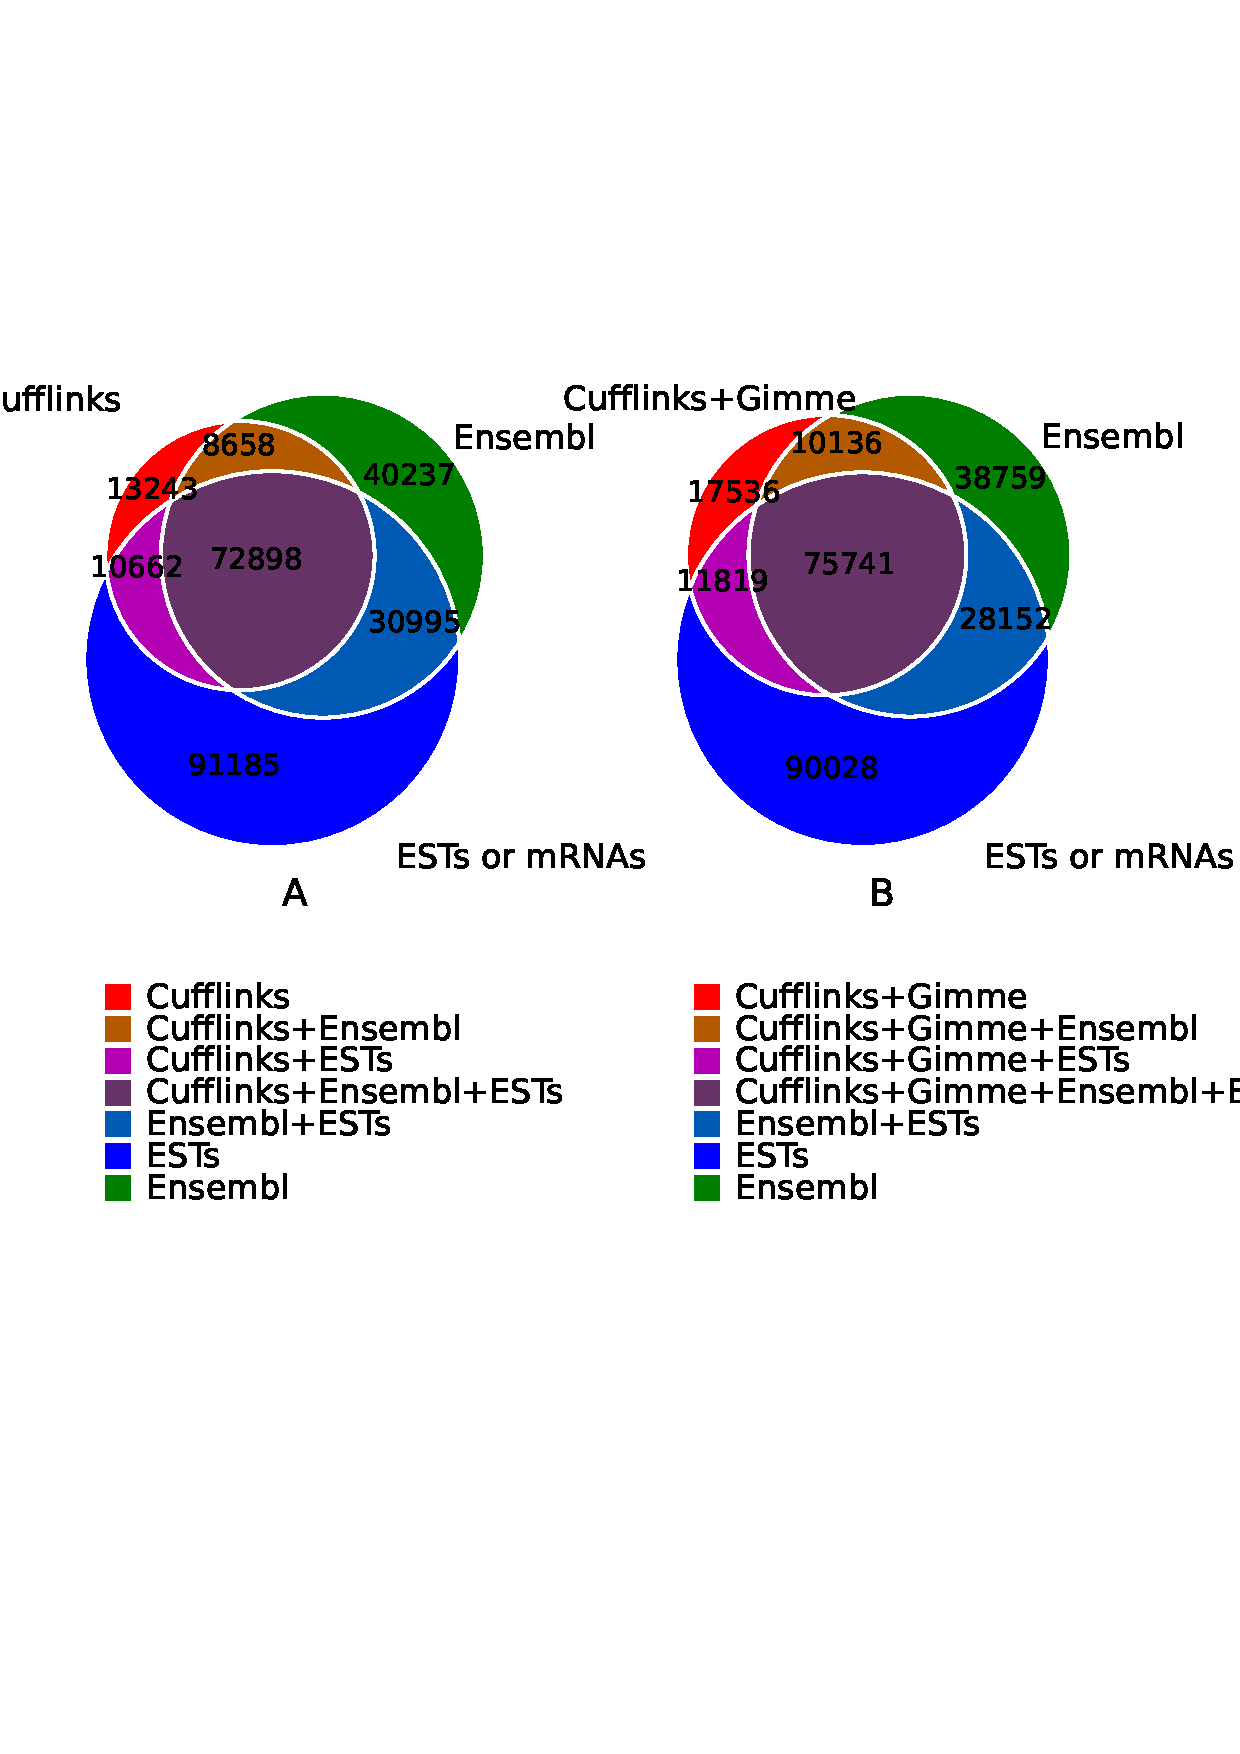
\includegraphics[width=8in]{cuff_gimme_junctions_venn.pdf}
\end{center}
\caption{
    \textbf{Splice junctions found in merged models.} Merged models (B) find more
    splice junctions in Ensembl and ESTs + mRNAs than Cufflinks models only (A).
}
\label{combined_venn}
\end{figure}
\end{landscape}
\pagestyle{plain}

\subsubsection{Validating chicken sequences by using mouse homologs}

To validate our predicted isoforms, we extracted putative coding
sequences from our gene models with ESTScan~\cite{Iseli:1999vd}.
ESTScan successfully translated 28,772 of 34,800 (82.6\%) of our
isoforms to protein sequences with 50 or more amino acids.  We
then searched for homologous sequences in mouse Ensembl, and
found that 22,991 (79.9\%) of our isoforms from 12,945 distinct
genes match mouse proteins at a bit score
$\ge1.0$(Figure~\ref{bitscore}).  These matches have a
bit-score/length ratio greater than 1, which indicates a good
agreement between chicken and mouse proteins.

\begin{figure}[!ht]
\begin{center}
\includegraphics[width=6in]{mouse-homolog-boxplot.pdf}
\end{center}
\caption{
\textbf{Box plots of bit score/length ratio of isoforms and genes that match mouse
proteins.}
}
\label{bitscore}
\end{figure}

% @CTB for discussion: what's surprising about all of this? so many
% splice variants, etc?  Note we need to go over pickrell paper carefully.

\section{Discussion}

For organisms with a reference genome and Ensembl annotation, building gene
models from RNA-Seq reads using Cufflinks with Ensembl gene models as a
reference guide seems to be a preferable method for gene and isoform expression
analysis.  However, we have shown that Ensembl models in chicken are missing a
substantial number of splice variants found in ESTs and mRNAs and Cufflinks does
not recover all splice variants.  A previous study by Schulz \emph{et
al.}~\cite{Schulz:2012je} demonstrated that Cufflinks outperformed \emph{de novo}
assembly in detecting genes and isoforms in Ensembl annotations in mouse.
However, we found that Cufflinks almost exclusively finds splice junctions in
mouse Ensembl gene models whereas our gene models include splice junctions not in
Ensembl gene models but supported by ESTs (Figure~\ref{mus_venn}). 

To build mouse Cufflinks gene models, we used Tophat default parameters claimed
to be fine-tuned for mammalian RNA-Seq reads, but Cufflinks still poorly
detected splice junctions not in Ensembl.  This suggests that the parameters may
have been set based on mammalian Ensembl models, which could limit the
efficiency of finding novel splice variants in other non-mammal organisms.  In
contrast, {\em de novo} assembly does not rely on species-specific parameters.
It is, therefore, recommended that a combination of Cufflinks models and
transcripts from {\em de novo} assembly should be used to build gene models that
include more splice variants.

We have also shown that the local assembly could greatly increase sensitivity
of splice variant detection. However, how the local assembly affects the
assembly process is not clearly understood.  We speculate that reads with
multiple alignments may play a significant role in enhancing the assembly of
splice variants.  Understanding of the mechanisms may lead to a technique that
can be applied to find splice variants in organisms that lack a reference
genome.

Both Cufflinks and our pipeline rely heavily on a reference genome; therefore,
the quality of the genome will greatly affect the quality of the gene models.
In this study gene models were built from chicken genome version 2.1 (galGal3),
which contains ~17 Mb of sequence duplications and missassemblies
that were eliminated in the latest version of genome assembly
(galGal4).  Duplications and misassemblies lead to false splice junctions, which
in turn produce a large number of splice variants as observed in some
chromosomes.

\section{Materials and Methods}

\subsection{Reads quality trimming}
Both single- and paired-end reads in this study were trimmed using Condetri
version 2.1 with default parameters.  In addition, the first 10 bases of each
reads were trimmed off due to an inconsistency of base-calling.

\subsection{Data}
Mouse RNA-Seq dataset (SRX062280) is downloaded from Short Read Archives (SRA).
Chicken RNA-Seq datasets were obtained from sequencing of mRNAs from spleen of
chicken line 6 and 7.

\subsection{Mapping reads to the genome and gene models}

Single and paired-end reads were mapped to the chicken genome by
Tophat~\cite{Trapnell:2009dp} release 1.3.1 using default
parameters without annotations.  All reads were mapped to cDNA
sequences derived from gene models by
Bowtie~\cite{Langmead:2009fv} release 1.0.0 with default
parameters.  Reads from the mouse dataset were mapped to the
mouse genome (mm9) downloaded from Tophat website

\texttt{http://tophat.cbcb.umd.edu}.

\subsection{Global and local assembly}

Reads from each dataset were first assembled separately by global assembly
without using a reference genome.  In contrast, reads from each dataset were
first mapped to the chicken genome using Tophat2.  Then only reads mapped to
the genome were assembled by chromosome in the local assembly
(Figure~\ref{local_assembly}).  Global and local assembly was performed using
Velvet version 1.2.03~\cite{Zerbino:2008vu} with default parameters except for
hash length (k-mer).  A range of k-mer length from 21-31 was used to assemble
reads from chicken data and k-mer length 27 was used to assemble reads from
mouse data.  Lastly, transcripts from both methods were assembled by Oases
version 0.2.06~\cite{Schulz:2012je}.  A poly-A tail, short transcripts and
transcripts with low complexity are removed by seqclean~\cite{seqclean} with
default parameters.  Redundant transcripts are removed by cd-hit-est from the
CD-HIT suite~\cite{Li:2006hr}.  A substantial number of transcripts are removed
at this step, which facilitates gene model construction process.

We obtained 339,199 transcripts, of which 315,998 transcripts (93.2\%) mapped
to chicken genome.  Only transcripts mapped to chicken genome are used to build
gene models.

\begin{figure}[!ht]
\begin{center}
\includegraphics[width=6in]{local_assembly}
\end{center}
\caption{
\textbf{Local Assembly Pipeline.}
Reads are first mapped to a chicken genome.  Then only mapped reads are
assembled by Velvet and Oases. Reads mapped to each chromosome
are assembled separately.
}
\label{local_assembly}
\end{figure}

\subsection{Gene model construction}
\subsubsection{Overall pipeline}

Figure~\ref{pipeline} depicts an overall gene model
construction pipeline.  Transcripts of all datasets from local
and global assembly were mapped to the chicken genome using
BLAT~\cite{Kent:2002tv}.  Alignments and gaps from BLAT outputs
are considered exons and introns respectively.  Optionally, data
from other sources (ESTs, RefGenes, Cufflinks, Ensembl and etc.)
can be incorporated with transcripts from the assembly to improve
gene models.  All transcripts are then assembled using Gimme, a
program that assembles transcripts based on their alignments to
the reference genome.  An algorithm for assembling transcripts is
described below.  A maximum set of transcripts obtained from
Gimme are then reduced to only a minimum set of transcripts that
contain all splice junctions and untranslated regions (UTRs).
After that, transcripts that are highly similar ($>99\%$) are
clustered and removed by CD-HIT version 4.5.6~\cite{Li:2006hr}.
Only a representative of each cluster is kept in gene models.

\begin{figure}[!ht]
\begin{center}
\includegraphics[width=5in]{pipeline.pdf}
\end{center}
\caption{
\textbf{Gene model construction pipeline.} Transcripts are obtained from two
assembly methods -- global and local assembly.  Transcripts are aligned to the
chicken genome by BLAT. Gimme then constructs gene models based on alignments
of transcripts. Gene models from Cufflinks can also be
incorporated to build the gene models.}
\label{pipeline}
\end{figure}

\subsubsection{Algorithm}

A gene model can be represented as a splice graph composed of exons as nodes and
introns as edges.  However, transcripts of the same gene vary in size and
structure depending on the expression level and a hash length number used in
the assembly.  Furthermore, incomplete exons and fragmented transcripts complicate
the construction of a splice graph.  In this study, we developed an algorithm
that handles incomplete exons and fragmented transcripts and constructs a
maximum assembly of gene models.

The algorithm first builds an intron graph using introns as nodes.  Each intron
contains exons one of whose splice sites perfectly match intron boundaries.
Exons are considered incomplete and eliminated if they locate at the $3'$ or
$5'$ end of the transcripts and they are not the largest exons
(Figure~\ref{algorithm}).  Transcripts were then grouped into the same gene if
they have at least one intron or exon in common.  Then, a splice graph composed
of exons is created and structures of isoforms are derived from traversing
paths in the splice graph.  Gimme is open-source and available at
\texttt{https://github.com/ged-lab/gimme}.

\subsection{Protein sequence translation}

We employed ESTScan version 3.0.3 to translate protein sequences from our gene
models.  The matrix used for building Hidden Markov models was built from chicken
reference cDNA sequences using tools from ESTScan. Only protein sequences longer
than 50 bp are included in the analysis.

\subsection{Finding unique sequences between datasets}

To identify unique sequences from two datasets, a set of 20-mers is created for
both datasets using khmer.  Then, 20-mers from a query dataset are
compared with 20-mers from the target dataset.  The sequence is considered
unique if more than 90\% of 20-mers in the query is unique.  Any unique region
shorter than 300 bp is ignored.

\subsection{Sequence homology analysis}

Protein sequences translated from each isoform using ESTScan were searched
against mouse reference proteins by BLAST 2.2.25+~\cite{Tatusova:1999tz}.  A bit
score to a length ratio was calculated for each hit that had an e-value $\le$
10\textsuperscript{-20}.  Only the highest value of all isoforms from each gene
was shown in the gene plot; whereas, values of all isoforms were shown in the
isoform plot.

\subsection{Spliced reads count}

Reads from each dataset were mapped to transcripts from the gene models using
Bowtie version 1.0.0. The parameter is set for Bowtie to report up to 100
alignments per read.  Reads mapped across exon junctions from all datasets were
counted using Samtools~\cite{li2009sequence} and Pysam~\cite{pysam}.

\subsection{Sequence assembly using Cufflinks}
Reads are mapped to a genome sequence using Tophat.  Gene models are built from
each dataset by Cufflinks 2.0.0~\cite{Trapnell:2010kd}.  All gene models are
then merged together using Cuffmerge.

\subsection{Expressed sequence tags and Genbank mRNA}
Expressed sequence tags (ESTs) and mRNAs were downloaded from the UCSC genome
website.  The database was loaded from GENBANK on 1 January 2014.  Sequences
were aligned to the chicken genome using BLAT.

\subsection{Pipeline and Scripts}

The pipeline and scripts used in this study is hosted at

\texttt{https://github.com/likit/gimme\_protocols}

\chapter{Comparison of Gene Network Inferred by RNA-Seq analysis}
\section{Introduction}

Differential expression (DE) and pathway analysis are widely used
techniques to identify candidate genes and pathways associated with
phenotypes or diseases~\cite{smith2011systems,beane2011characterizing,
  li2012rna}.  The advent of high-throughput technologies such as
microarrays and next-generation sequencing (NGS) has led to an
explosion of tools and pipelines for exploring expression data.  Most
of the tools for DE and pathway analyses rely on publically
available gene sets such as Ensembl for quantification of gene
expression and downstream pathway annotation.

% @CTB maybe move, maybe keep, not sure yet :)
%Ensembl gene models are maintained and updated by the Ensembl project
%(\texttt{http://ensembl.org}), which provide gene annotations for 70
%species~\cite{flicek2013ensembl}.  The annotations are linked to
%external information such as gene names from HUGO Gene Nomenclature
%Committee (HGNC), the Protein Databank (PDB), the Universal Protein
%Resources (UNIPROT), the RefSeq collection of Reference Sequences, and
%the UCSC Genome Browser. These annotations include evidence taken from
%tissue-specific RNA-Seq data.  This provides a great resource for
%studying tissue-specific gene expressions as well as alternate splice
%forms.  KEGG pathway is a reference knowledge base that provides
%information for understanding higher-level functions of cellular
%processes and organism behaviors; it is maintained at
%\texttt{http://www.genome.jp/kegg}. These publically available
%information resources have been extremely useful for biologists in the
%genomic era, especially those who study model organisms such as human
%and mouse.

Recently, RNA sequencing (RNA-Seq) by NGS technology has not
only allowed biologists to study expression of annotated
genes but also to discover novel genes and isoforms as well
as to obtain evidence of transcribed but untranslated
regions~\cite{pickrell2010understanding,
lu2010function,otto2010new,raghavachari2012systematic}.
This technology also provides an opportunity for biologists
to generate more comprehensive transcriptomes for organisms
by reconstructing transcript sequences from short reads
using \textit{de novo} assembly or \textit{ab initio}
methods.  However, because executing these tools requires
significant computational expertise, researchers may rely on
existing annotation resources instead of building new gene
models.

The consequences of using different gene models on gene
expression analysis and pathway predictions have not been
explored.  We speculated that more comprehensive gene models
could affect these analyses significantly, especially in
organisms where the available gene annotations are
relatively sparse compared to NIH model organisms.
Incomplete gene models are insensitive to read mapping,
which would affect predicted gene expression levels and the
significance of differential expression calculations; in
addition, missing splice variants and exons limit the power
of differential isoform expression analysis.  Missing gene
models also decrease the power of GO and KEGG pathway
analyses by potentially eliminating genes important for
pathways.

In this article, we present comparisons of differential
expression computations and KEGG pathway analyses of RNA-seq
data between Ensembl gene models, {\em ab initio} and {\em
de novo} constructed gene models, and merged gene models
built from all of the above.  We also show the effect on
predictions of differentially expressed pathways when
including KEGG pathway annotations from human in our
analysis.  We demonstrate that the gene models used and the
extent of the annotation source significantly affect
predictions and their statistical support.  Finally, we
discuss the implications for the investigation of organisms
with relatively incomplete gene annotations.

% Results and Discussion can be combined.
\section{Results}

\subsection{The set of differentially expressed genes varies widely
by gene model set used}

% @CTB: side note, make sure we discuss ``why rsem?'' and ``are our results
% general beyond RSEM?'' down below, in dsicussion

The first step in pathway enrichment analysis is to identify
differentially expressed genes.  Starting with each of four
different sets of gene models, we used RSEM to estimate gene
expression and then applied EBSeq to identify differentially
expressed genes.  For gene models, we used the public
Ensembl gene models together with three sets of custom gene
models.  The custom-constructed gene models were, (1)
constructed by {\em de novo} mRNAseq assembly with
Velvet/Oases~\cite{Zerbino:2008vu,Schulz:2012je}, (2) a
genome reference-guided gene set constructed with
Cufflinks~\cite{Trapnell:2010kd}, and (3) a merged gene set
constructed with Gimme from a combination of all three other
gene sets; see Methods for details.  All custom gene sets
were constructed using the same Marek's Disease Virus
mRNAseq data sets used for differential expression analysis.

We next examined the rate of read mapping to the gene
models.  The percentages of reads mapped to the Ensembl
models are lowest in all samples compared to other gene
model sets (Table ~\ref{tab:mapped-reads}).  Fewer than 60\%
of reads mapped to the Ensembl models indicating that the
gene models do not include all coding and non-coding regions
expressed in the samples.  The results from the assembly
models confirm that many reads are from regions not included
in the Ensembl models. Note that the number of mapped
single-end reads is highest in the assembly models, even
though those models have the fewest distinct genes.

\begin{table}[!ht]
\caption{
\textbf{Rate of reads mapped to Ensembl-matched gene models}
}
\begin{center}
\begin{tabular}{ccccccc}
\hline
& Single & & Paired-end & & Total & \\
& Control & Infected & Control & Infected & Genes \\
\hline
Ensembl & 61.93\% & 63.59\% & 57.83\% & 59.24\% & 15,943 \\
Assembly & 81.40\% & 84.01\% & 64.24\% & 66.75\% & 9,002 \\
Cufflinks & 78.16\% & 81.28\% & 76.56\% & 77.44\% & 14,020 \\
Merged & 78.14\% & 81.48\% & 75.87\% & 77.23\% & 13,973 \\
Total reads & 27,618,789 & 29,693,654 & 42,632,733 & 30,804,398 & \\
\hline
\end{tabular}
\end{center}
%\begin{flushleft}
%    (-) down-regulated, (+) up-regulated
%\end{flushleft}
\label{tab:mapped-reads}
\end{table}
% However, the number of mapped
%paired-end reads are more reliable due to stringency of paired-end
%mapping criteria.
% @CTB: Likit, were the paired-end reads used to construct the
% gene models?
% @Likit: Yes.

We compared differentially expressed gene predictions
between data sets by linking each gene to an Ensembl gene
via BLAST, which provided a common reference identifier.  A
summary of the correspondence is in
Table~\ref{tab:ensbl_matched}.  From {\em de novo} assembly,
9002 (56.46\%) of the gene models matched to one of the
approximately 16,000 Ensembl genes.  Cufflinks and merged
models matched considerably more of the Ensembl genes --
14020 (87.9\%) and 13973 (87.6\%), respectively.

\begin{table}[!ht]
\caption{
\textbf{Genes and DE genes matched Ensembl genes}}
\begin{center}
\begin{tabular}{ccccc}
\hline
& Ensembl & Assembly & Cufflinks & Merged \\
\hline
All & 15943 & 9002 & 14020 & 13973 \\
DE & 2538 & 2109 & 3433 & 3402 \\
\hline
\end{tabular}
\end{center}
%\begin{flushleft}
%    (-) down-regulated, (+) up-regulated
%\end{flushleft}
\label{tab:ensbl_matched}
\end{table}

Of the genes in the different data sets with identifiable
correspondence to Ensembl, RSEM predicted that between 2109
and 3433 genes were differentially expressed (DE) across the
gene model sets.  However, the number of DE genes shared
between two different gene sets was much lower, with a
maximum of 3069 out of 3428 (89.5\%) DE genes shared between
Gimme and Cufflinks (Figure~\ref{degenes_venn}D).  Gimme
incorporates the Cufflinks gene models, however, and so the
best agreement on DE genes between two independent data sets
is between Ensembl and Cufflinks, where 1991 genes are DE in
both Ensembl (1991 of 2538 DE genes, 78.4\%) and Cufflinks
(1991 of 3428, 58.0\%).  Despite this correspondence, the
number of disjoint DE genes between samples is often equal
to or larger than the number of DE genes in common between
any two gene sets.

\begin{figure}[!ht]
    \begin{center}
        \includegraphics[width=6in]{ensbl-assm-cuff-comb-degenes-venn.pdf}
    \end{center}
    \caption{
        \textbf{Comparison of differentially expressed genes.}
        DE genes were matched to Ensembl genes via BLAST. (A-C) The number of DE
        genes in other gene model sets differ greatly when compared to Ensembl
        models.  (D) Although Cufflinks models were incorporated into Gimme
        models, not all DE genes in Cufflinks were found in Gimme models.
    }
    \label{degenes_venn}
\end{figure}
% @CTB can you do a venn diagram as in Eli's paper for this, do you think?
% @LP I will look at it.

\subsection{Variation in differential expression predictions is due to
variation in read mapping}

To identify the factors contributing to variation in DE
analysis, we examined estimated read counts of genes
identified as differentially expressed in one gene model set
versus another.  For example, the {\em IFNB} gene was not DE
when the Ensembl models were used, but was DE when the
merged Gimme models were used; upon examination, we found
that the number of reads mapping to the {\em IFNB} gene
model was much higher in the merged models
(Figure~\ref{ifnb_count}).  This discrepancy in mapped reads
was due to a substantial number of reads mapped to the
extended regions in the Gimme model, which are not included
in the Ensembl model (Figure~\ref{ifnb}).  Another example
is the {\em IDH3A} gene, shown in Figure~\ref{idh3a}. This
gene was expressed in both control and infected groups, but
is only identified as DE when the Gimme models are used
(Figure~\ref{idh3a_count}).  This is because the complete
$5\prime$ UTR is included in only one of the two Ensembl
isoforms and not in the RefSeq model, whereas both $3\prime$
and $5\prime$ UTRs are included in the Gimme model.  The
size of the $3\prime$ UTR in the Gimme model is slightly
larger than that of RefSeq and the size of the Gimme
$5\prime$ UTR is the same as that of Ensembl model.

\begin{figure}[!ht]
    \begin{center}
        \includegraphics[width=6in]{ifnb-raw-reads-bar.pdf}
    \end{center}
    \caption{
        \textbf{Read counts of {\em IFNB} gene.} SE=single-end, PE=paired-end
    }
    \label{ifnb_count}
\end{figure}

\clearpage\pagestyle{lscape}
\begin{landscape}
\begin{figure}[!ht]
    \begin{center}
        \includegraphics[width=8in]{ifnb.pdf}
    \end{center}
    \caption{
        \textbf{{\em IFNB} gene models from Ensembl
        (ENSGALT00000039477, red), Gimme (chrZ:34927.1, black)
        and RefSeq (blue).}
        RefSeq and Ensembl models only include the CDS region;
        whereas, Gimme model include extended regions that could
        be unstranslated regions (UTRs). The extended regions are
        of notable sizes, which could account for a substantial
        number of mapped reads.
    }
    \label{ifnb}
\end{figure}

\begin{figure}[!ht]
    \begin{center}
        \includegraphics[width=8in]{idh3a.pdf}
    \end{center}
    \caption{
        \textbf{{\em IDH3A} gene models from Ensembl
        (ENSGALT00000005233,39672, red), Gimme
        (chr10:7977.1, chr10:7977.2, black) and RefSeq (blue).}
        RefSeq model only includes CDS and $3\prime$ UTR. Ensembl
        model only includes CDS and $5\prime$ UTR in one isoform.
        Gimme model includes CDS and both UTRs.
    }
    \label{idh3a}
\end{figure}
\end{landscape}
\pagestyle{plain}

\begin{figure}[!ht]
    \begin{center}
        \includegraphics[width=6in]{idh3a-raw-reads-bar.pdf}
    \end{center}
    \caption{
        \textbf{Read counts of {\em IDH3A} gene.} SE=single-end, PE=paired-end
    }
    \label{idh3a_count}
\end{figure}

We next examined the gene size distribution across all four
gene model sets used (Figure~\ref{gene_length}).  Both the
Cufflinks {\em ab initio} gene models and the Gimme merged
gene models are significantly longer than the Ensembl and
assembly-based gene models, suggesting that they are more
complete.

% \pagestyle{empty}
% \begin{landscape}
\begin{figure}[!ht]
    \begin{center}
        \includegraphics[width=6in]{gene_length.pdf}
    \end{center}
    \caption{
        \textbf{Gene sizes distribution.}
        Distribution of the same set of genes from different models are plotted.
        Sizes of genes in Ensembl models are slightly shorter than those from
        combined models. This is due partly to the fact that some genes may not
        contain UTRs.
        The sizes of genes from \textit{de novo} assembly are significantly smaller
        than other models indicating that transcripts are incomplete or fragmented.
    }
    \label{gene_length}
\end{figure}
% \end{landscape}
% \pagestyle{plain}

Finally, we examined the read counts and length-normalized
read counts for control and infected mRNAseq samples
(Figure~\ref{read_count}). In all cases, both the read
counts and length-normalized read counts were significantly
higher for the Gimme gene models.

% \pagestyle{empty}
% \begin{landscape}
\begin{figure}[!ht]
    \begin{center}
        \includegraphics[width=6.5in]{read_count.pdf}
    \end{center}
    \caption{
        \textbf{Read counts comparisons.}
        In the same condition, read counts from Gimme models are significantly
        higher than those from Ensembl gene models.  Read counts are more
        similar after normalization by gene lengths.  Read counts were
        normalized by effective gene sizes using this formula: $1000 \times
        \frac{count}{length} = Read Per Kilobase (RPK)$.
    }
    \label{read_count}
\end{figure}
% \end{landscape}
% \pagestyle{plain}

To illustrate the effect of gene models variation on gene
expression estimates, comparisons of effective gene sizes
from all gene models and read counts from Ensembl and merged
models are shown in Figure~\ref{gene_length}
and~\ref{read_count}.  Effective gene sizes of 1,563
differential-expressed gene vary greatly among gene models
(Figure~\ref{gene_length}). The effective gene size is the
average of sizes of all transcripts from the same gene.  The
median of effective gene sizes of Ensembl models is 2413 bp
(IQR 2250 bp); whereas those of Cufflinks and merged models
are much higher (3320 bp (IQR 2550 bp) and 3270 bp (IQR 2595
bp) respectively).  This is expected because Cufflinks and
combined models are supposed to include UTRs.  On the other
hand, the median of the effective gene sizes of gene models
from {\em de novo} assembly is close to that of Ensembl
models; however, the IQR is much smaller (median = 2273 bp,
IQR = 1474 bp) suggesting that transcripts from \textit{de
novo} assembly are incomplete compared to Ensembl models.
The difference in gene sizes between Ensembl and combined
models results in a substantial deviation of read counts as
shown in Figure~\ref{read_count}.  Medians of read counts
from the same condition were significantly different between
Ensembl and combined models.  After normalization by gene
sizes, the difference were diminished suggesting that the
deviation of read counts is partly due to the size of the
gene models. 

\subsection{A majority of differential-expressed genes are
not annotated in KEGG pathway}

We next used the Kyoto Encyclopedia of Gene and Genomes
(KEGG) to annotate the differentially-expressed genes with
putative function and identify enriched pathways using
GOSeq~\cite{young2010method}.  Because there are only a
small number of species-specific chicken annotations in the
KEGG database, we also used homology search against human
Ensembl proteins (Release 74) to transfer gene annotations
from human genes to our chicken gene models.

Transferring gene annotations from human to chicken did not
result in a large increase in the number of genes that were
annotated, but the number of genes with pathway annotations
did increase.  In Figure~\ref{num_kegg}, we show the effect
of this transfer on the pathway annotations for different
gene model sets.
% LP the results below changed significantly. I might have
% done something wrong before.
For the merged data set, $\sim$27\% of DE gene models had
species-specific KEGG annotations, while approximately 36\%
had human KEGG annotations.

\begin{figure}[!ht]
    \begin{center}
        \includegraphics[width=6in]{gallus-hsa-num-kegg-genes-bar.pdf}
    \end{center}
    \caption{
        \textbf{DE genes with chicken and human KEGG annotations.}
    }
    \label{num_kegg}
\end{figure}

Unsurprisingly, transferring gene annotations also led to a
dramatic difference in the KEGG pathways predicted to be
enriched between the two conditions.
Figure~\ref{gimme_hs_ga} shows the enriched KEGG pathways in
the merged gene models with first, only chicken annotation
and second, with transferred human annotations.  A total of
26 pathways were predicted to be enriched in one or both of
the annotation sets, with 6 in common, 9 unique to the
species-specific annotations, and 11 unique to the human
annotation set.  A majority of the chicken-specific
annotations were immune system annotations, reflecting the
extensive work done on chicken
immunity~\cite{burt2005chicken}.

\subsection{Pathway predictions vary widely between gene
model sets}

To compare the pathway predictions using chicken+human
annotations, we calculated the Spearman rank correlation
coefficient for all possible pair-wise comparisons.  The results,
shown in Table~\ref{tab:spearmanr}, show that the correlations
are very poor.  The weakest correlation is between the pathway
predictions for the Ensembl gene model set and the merged gene
model set.

\begin{table}[!ht]
\caption{
\textbf{Spearman Rank Correlation}}
\begin{center}
\begin{tabular}{ccccc}
\hline
& Assembly & Ensembl & Cufflinks & Merged \\
\hline
Assembly & 1.0 & 0.39 & 0.45 & 0.50 \\
Ensembl & & 1.0 & 0.48 & 0.36 \\
Cufflinks & & & 1.0 & 0.76 \\
Merged & & & & 1.0 \\
\hline
\end{tabular}
\end{center}
%\begin{flushleft}
%    (-) down-regulated, (+) up-regulated
%\end{flushleft}
\label{tab:spearmanr}
\end{table}

% @CTB: what is the goal of these last two sentences? An
% example of how they are different.
Five pathways are predicted to be enriched only when using
the Ensembl gene models (Figure~\ref{KEGG_all}), including
the antigen processing and presentation pathway, which is
important for immune responses.  In addition, the T cell
receptor signaling pathway is predicted to be enriched in
all of the gene model sets excepting only the Ensembl
models.

The correlation coefficient between enriched pathways
predicted from Ensembl gene models and Cufflinks gene models
is rather high, which may be because the Ensembl models were
integrated with RNA-Seq data to construct the Cufflinks
models.  The integration is done based on the criteria that
incomplete transcripts or transcripts without novel introns
compared to the Ensembl models are discarded and UTRs from
RNA-Seq data are used to extend Ensembl UTRs
~\cite{roberts2011identification}.  Therefore, Cufflinks
models are a superset of the Ensembl models and should
contain all pathways from Ensembl models.  However, eighteen
pathways are unique to Cufflinks and seven pathways are
unique to Ensembl; this may be due to a difference in the
read mapping percentage.
% @CTB: or just statistics, right?  More genes, different
% cutoffs...

Finally, the correlation between enriched pathways predicted
using the Cufflinks-based differential expression and the
Gimme-based differential expression is the highest.
Although twelve enriched pathways are unique to Cufflinks,
and four pathways are unique to the merged models, the
correlation coefficient is high because the common pathways
have similar significance scores.  Twenty nine enriched
pathways are different between the merged models and Ensembl
and this results in a slightly lower correlation coefficient
than that between the combined models and Cufflinks.
Table~\ref{tab:combined_unique} shows common and unique
enriched pathways from Ensembl and combined models.  A
majority of unique enriched pathways from Ensembl are
involved in metabolism and cellular activities.
% @Jerry: the following paragrah is not an explanation
In contrast, unique pathways from combined models are
involved in immune response and cancer, which we would
expect to be perturbed by MDV infection.

\begin{table}[!ht]
\caption{
\textbf{Pathways from Ensembl and merged gene models}}
\begin{center}
\begin{tabular}{ccc}
\hline
pathway ID & Term & Adjusted p-value \\
\hline
& Pathways in Ensembl only & \\
\hline
00980 & Metabolism of xenobiotics by cytochrome P450 & 2.3e-06 \\
00480 & Glutathione metabolism & 1.9e-05 \\
00982 & Drug metabolism - cytochrome P450 & 9.5e-04 \\
04142 & Lysosome & 1.1e-03 \\
04010 & MAPK signaling pathway & 3.0e-03 \\
00400 & Phenylalanine, tyrosine and tryptophan biosynthesis & 3.4e-03 \\
00500 & Starch and sucrose metabolism & 4.9e-03 \\
00983 & Drug metabolism - other enzymes & 5.5e-03 \\
00360 & Phenylalanine metabolism & 6.3e-03 \\
\hline
& Common pathways & \\
\hline
04060 & Cytokine-cytokine receptor interaction & 5.8e-15 \\
04145 & Phagosome & 4.7e-07 \\
01100 & Metabolic pathways & 1.1e-06 \\
04620 & Toll-like receptor signaling pathway & 4.8e-05 \\
04623 & Cytosolic DNA-sensing pathway & 1.2e-04 \\
04210 & Apoptosis & 1.8e-04 \\
04630 & Jak-STAT signaling pathway & 2.1e-04 \\
04672 & Intestinal immune network for IgA production & 2.4e-04 \\
04622 & RIG-I-like receptor signaling pathway & 3.6e-04 \\
04621 & NOD-like receptor signaling pathway & 1.4e-03 \\
04650 & Natural killer cell mediated cytotoxicity & 2.0e-03 \\
\hline
& Pathways in merged models only & \\
\hline
04514 & Cell adhesion molecules (CAMs) & 1.8e-04 \\
04141 & Protein processing in endoplasmic reticulum & 10.0e-04 \\
04510 & Focal adhesion & 2.3e-03 \\
04512 & ECM-receptor interaction & 3.3e-03 \\
\hline
\end{tabular}
\end{center}
\begin{flushleft}
\end{flushleft}
\label{tab:combined_unique}
\end{table}

% @CTB: this text belongs in either introduction or
% discussion, not in results!
For non-model organisms without high-coverage functional
pathway annotation or gene ontology (GO), an alternative
method for functional analysis is to use pathway annotations
of closely related or well-studied model organisms such as
mouse and human.  This approach could increase
sensitivity of pathway analysis; however, it will not
include species-specific genes and pathways.  For instance,
in this study, some pathways involved in chicken immune
responses including natural killer cell mediated
cytotoxicity, intestinal immune network for IgA production,
and focal adhesion were not enriched in human annotation
with merged models (Figure~\ref{gimme_hs_ga}).

\begin{figure}[!ht]
    \begin{center}
        \includegraphics[width=6in]{gimme-hsa-gga-kegg-pvalue-bar.pdf}
    \end{center}
    \caption{
        \textbf{Enriched KEGG Pathways from merged models with
        chicken and human annotation}
    }
    \label{gimme_hs_ga}
\end{figure}

To overcome this problem, we propose to use a custom pathway
annotation built from a combination of annotations from the
organism and related species.  To validate our method, we
built a custom annotation by assigning human annotations to
chicken genes with no pathway annotations and used the
custom annotation for pahtway analysis.  The results (shown
at the bottom graph of Figure~\ref{KEGG_all}) include some
significantly enriched pathways involved in immune responses
such as complement and coagulation cascades, T cells
receptor pathway, and chemokines signaling pathway. Almost
all enriched pathways from either Cufflinks or Ensembl
models are also included.  Besides the top three most
significant pathways, pathways from custom annotations,
Cufflinks and Ensembl have only slightly different
significance scores.  This indicates that custom annotation
can help increase the sensitivity of pathway analysis,
especially in semi-model organisms.  However, results have
to be interpreted with great care due to biological
differences between organisms.

\begin{figure}[!ht]
    \begin{center}
        \includegraphics[width=6in]{gallus-kegg-pvalue-bar.pdf}
    \end{center}
    \caption{
        \textbf{Enriched KEGG Pathways from different gene models}
    }
    \label{KEGG_all}
\end{figure}

\section{Discussion}

\subsection{Variation in gene model sets greatly affects expression estimates}

Methods for differential gene expression analysis typically
estimate gene expression from the number of reads mapped to
each gene model.  Reads that do not map to gene models, such
as reads belonging to unannotated UTRs or exons, are
generally excluded.  This exclusion leads to insensitivity
in estimates of expression, and can be particularly
problematic when genes have long UTRs and uenven read
coverage.

Here, we show that using the same parameters for mapping and
differential exprssion analysis with several different gene
model sets results in large differences in both read mapping
and the prediction of differentially expressed (DE) genes.
While some differences are expected, we found that the
differences were surprisingly large: for most of the
comparisons, the DE genes disjoint between the two gene
model sets were larger in number than the DE genes shared
between the two gene model sets.

These differences are due to differences in the number of
reads mapping to the gene models.  Unsurprisingly, many more
reads map to the gene model data sets constructed from the
mRNAseq data -- between 15\% and 20\%
(Table~\ref{tab:mapped-reads}).  This results in many more
reads mapping to each gene model (Figure~\ref{gene_length}a)
and significantly higher RPKM estimates for each mRNAseq
data set (Figure~\ref{gene_length}b).

\subsection{Conclusion}

As the use of RNA-Seq to study semi- and non-model organisms
has vastly increased recently, one objective of this study
is to demonstrate the potential problem of transcriptome
study in organisms that lack high quality genome, gene
models and functional pathway annotation.  Gene models
derived from {\em de novo} assembly are usually the only
choice for those organisms; however, the results are
relatively poor compared to others.  Custom gene models
built from Cufflinks (integrated with Ensembl) helped
increase sensitivity of pathway analysis and should be used
if a reference genome is available and {\em de novo}
assembly is not feasible.  However, the method is reliant on
a quality of a genome sequence and subject to read-mapping
biases.  Combined gene models, although appearing to have
lower sensitivity compared to those from Cufflinks and
Ensembl, still recover most of the pathways with high
significance scores.  The advantage of using combined gene
models is it allows the integration of gene models from {\em
de novo} assembly, which are not affected by read-mapping
biases.  Results from our study show that they significantly
increase sensitivity of genes and isoforms
detection.  Depending on available resources and the
objective of the study, we suggest that appropriate gene
models should be carefully chosen to maximize the quality of
the analysis.  Moreover, using functional pathway annotation
from a related species is always necessary for those
organisms, but it will not include species-specific genes
and pathways. The problem is compounded when only gene
models from {\em de novo} assembly are available. Therefore,
biologists studying non-model organisms need to be aware of
these limitations when interpreting the results from
transcriptome analysis.


% You may title this section "Methods" or "Models". 
% "Models" is not a valid title for PLoS ONE authors. However, PLoS ONE
% authors may use "Analysis" 
\section{Materials and Methods}

\subsection{Sequences and quality trimming}

mRNAs were extracted from spleens of control and infected
line 7 chickens (14 dpi).  Sequence libraries were prepared
by standard Illumina unstranded single- and paired-end
protocols.  Library size of the paired-end datasets is
approximately 175 bp.  Read lengths are 75 bp in both
single- and paired-end libraries.  Reads were quality
trimmed by condetri 2.1~\cite{smeds2011condetri} with
quality score cutoff of 30.  The first 10 bases were removed
due to a non-uniform distribution of nucleotides.

\subsection{Custom gene models construction}

Reads were mapped to chicken genome (galGal4) by TopHat
2.0.9~\cite{Trapnell:2009dp} and gene models were
constructed with Ensembl models release 73 as a reference by
Cufflinks 2.1.1~\cite{Trapnell:2010kd}.  Velvet
1.2.03~\cite{Zerbino:2008vu} and Oases
0.2.06~\cite{Schulz:2012je} were used to assemble reads with
hash lengths ranging from $21-31$.  Transcripts from all
hash lengths were then reassembled with OasesM.  Combined
gene models were constructed by Gimme~\cite{gimme:Online},
which combined Cufflinks models and alignments of \textit{de
novo} transcripts to the genome.  Transcripts were mapped to
the genome using BLAT~\cite{Kent:2002tv} and for each
transcript, only an alignment with the best mapping score
was used.


\subsection{Differential gene expression and gene ontology}

Quality filtered reads were mapped to transcripts from all
gene models without poly-A tail added by Bowtie
1.0~\cite{langmead2009ultrafast}.  Estimated gene expression
and differential expression analysis was performed by RSEM
1.2.7~\cite{li2011rsem} and EBseq~\cite{leng2013ebseq}
respectively.  DE genes were annotated by homologous
sequences in chicken and human proteins from Ensembl release
73 and 74 respectively.  GOSeq 1.14.0~\cite{young2010method}
was used to perform enrichment analysis using KEGG
annotations from org.Gg.eg.db~\cite{Gg} and
org.Hs.eg.db~\cite{Hs}.  Human KEGG annotations were added
to all DE genes to create combined KEGG pathways.

\subsection{Pipeline and scripts}

The pipeline and scripts used in this study is available at

\texttt{https://github.com/likit/RNASeq-methods-comparison}

\chapter{A genome-wide scan for genes and isoforms responsible
for MD resistance}
\section{Introduction}

Marek's disease (MD) is an economically significant chicken
disease that affects the poultry industry worldwide with
estimated annual cost of \$2 billion~\cite{morrow2004marek}.  The
disease is caused by the highly oncogenic Marek's disease virus
(MDV), an alphaherpesvirus that induces T-cell lymphomas in
susceptible birds.  Vaccination is the primary control measure,
which is effective in reducing incidence of tumor formation.
However, since MD vaccines are not sterilizing, they do not
prevent infection or horizontal spread of the virus.  As a
consequence, MDV field strains that overcome vaccinal protection
have arisen repeatedly over time.  Therefore, there is a need for
sustainable alternative controls measures, such as improving
genetic resistance.

Many studies have reported strong associations between MHC alleles and
resistance or susceptibility to MD.  For example, chickens with MHC
allele B\textsuperscript{21} are resistant in contrast to chickens
with the B\textsuperscript{19} allele, which are susceptible.  ADOL
lines 6 and 7, both share the same MHC B\textsuperscript{2} allele,
yet exhibit different phenotypic responses; e.g., challenge with the
JM/102W strain typically result in 0 and 100\% MD incidence for lines
6 and 7, respectively.  Thus, the major unanswered questions are what
genetic factors, especially those that are non-MHC, contribute to
susceptibility and resistance to the disease and what are the main
contributing mechanisms.

In the past decades, significant efforts have been made to study
variations in global gene expression between resistant and
susceptible birds using microarray and RNA-Seq methods in order
to identify non-MHC genes that contribute to resistance to
MD~\cite{sarson2008transcriptional,morgan2001induction,vallejo1998genetic,yonash1999high,bumstead1998genomic}.
However, none of the studies have investigated differential
expression of alternative isoforms, which are known to play a
significant role in many biological events including immune
responses.  In addition, studies have shown that isoform
expression levels can provide better signatures for some
diseases~\cite{zhang2013isoform}.  Changes of isoform expression
levels are governed partly by two types of {\em cis-}regulatory
elements: Exon Splicing Enhancer (ESE) and Exon Splicing Silencer
(ESS), which are located within an exon sequence.  A number of
sequence motifs of ESE and ESS have been identified in human and
some other organisms and can be predicted {\em in silico}.
Mutations that disrupt or create those motifs could alter
splicing patterns leading to aberrant alternative splicing.  A
number of disease-associated single-nucleotide polymorphsims in
coding regions (SNPs) that affect ESEs and ESSs have been well
characterized~\cite{blencowe2000exonic, wang2007splicing}.
%In fact, 15\% of mutations that cause genetic diseases affect
%pre-mRNA splicing via this mechanism.
Therefore, variations in isoform expression could lead to
identification of SNPs that underlie genetic resistance to MD.
In this article, we reported differential-expressed genes and
isoforms that may contribute to resistance to MD as well as SNPs
that can potentially affect isoform expression levels.

% Results and Discussion can be combined.
\section{Results and Discussion}

\subsection{Differential expression results from our method are
comparable to previous studies}

To study gene and isoform expression, we incorporated Ensembl gene
model release 73 with {\em de novo} and a reference-guided
transcriptome assembly to build custom chicken gene models.  The
models, therefore, include both Ensembl annotated transcripts and
putative genes and isoforms.  The advantage of using custom
gene models is it allows an investigation of unannotated genes and
isoforms, which is necessary for in-depth study of gene expression.

Some DE genes that were reported by previous microarray studies were
also found to be differentially expressed in this study.  For example,
B6.1 (Bu-1) is known to be down regulated approximately 2.3 fold in
susceptible chickens with the MHC allele B\textsuperscript{19} at 4
days post infection (d.p.i)~\cite{sarson2008transcriptional}.  It was
also found to be down regulated $\sim$3-fold in the susceptible line
in our study.  Similarly, {\em GMZA} reported to be upregulated across
genetically different chickens (B\textsuperscript{19},
B\textsuperscript{21} alleles), and was also found to be highly
upregulated here.  In contrast, some genes that have been reported to
be highly expressed in resistant chickens were downregulated in both
lines. Those genes are {\em AMIGO2, MMP13} and {\em CLEC3B}, which
were found to be downregulated more than
2-fold~\cite{sarson2008transcriptional}.
Other immune genes reported to be highly expressed in susceptible
chickens including {\em AVD, ART1, NOS2, CXCL13L2, MX1} and {\em
SOCS1}~\cite{smith2011systems} were also found to be highly
upregulated in both lines.  However, our results show a similar
expression patterns for {\em IL6} and {\em IL18}, which were only
upregulated in the susceptible line at an early stage of infection
($3-5$ d.p.i).

In contrast, {\em IL15} has been reported to be non
differentially expressed between control and infected chickens in
both lines~\cite{kaiser2003differential}; however, here it was only
upregulated in the susceptible line.  Expression of {\em IL15} is
induced by {\em TLR9}, which binds to non-methylated CpG residues
present in the genomes of many DNA viruses, including herpes simplex
virus.  This cytokine auto-regulates the expression of {\em
CD40}, which is a transmembrane receptor required for activation
of macrophages by CD4 T cells.  Consequently, {\em CD40} was only
upregulated in the susceptible line (data not shown).

\subsection{Differential gene expression indicates active immune
responses to ongoing lytic infection in the susceptible line}

Many genes were found to be differentially expressed (DE) between
control and infected chickens in both lines.  While the number of
unique downregulated genes in both lines was approximately equal,
the number of unique upregulated genes in the susceptible line
was much greater compared to the resistant line
(Figure~\ref{degenes_venn_diagram}).

\begin{figure}[!ht]
    \begin{center}
        \includegraphics[width=6in]{degenes_venn.pdf}
    \end{center}
    \caption{
        \textbf{Differential-expressed genes in response to MDV
        infection.}
        More genes are differentially expressed between control
        and infected chickens from line 7 than line 6.
    }
    \label{degenes_venn_diagram}
\end{figure}

Interestingly, some genes that were differentially expressed in
both lines were regulated in the opposite direction
(Table~\ref{tab:opposite}).  Among genes downregulated in the
resistant line but upregulated in the susceptible line were {\em
LL} (lung lectin) and {\em SFTPA1}, which encode a
calcium-dependent C-type lectin and a lung surfactant protein
respectively.  Both molecules are important in innate
immunity~\cite{hogenkamp2008chicken,kingma2006defense}.  {\em
LIMS1} is involved in cell differentiation and proliferation and
{\em PPARG} is a suppressor of the {\em NF$\kappa$B}-mediated
proinflamatory response.  On the other hand, nearly all genes
upregulated in the resistant line but downregulated in the
susceptible line are involved in cell survival such as mRNAs
splicing, cell growth, and protein synthesis, except CD7 whose
function is involved in T cell-B cell interaction.  This
difference suggests that even at this stage of infection in the
resistant line, the lytic phase could be repressed. Therefore,
only genes involved in cell division are upregulated possibly to
repair the initial damage due to infection in the resistant line.
In comparison, the lytic phase in the susceptible line may still
continue and as a result, genes involved in immune responses are
still upregulated.

\clearpage\pagestyle{lscape}
\begin{landscape}
\begin{table}
\caption{
\textbf{Genes regulated in opposite directions in response to MDV
infection}
}
\begin{center}
    \begin{tabular}{cccc}
        \hline
        Gene & Description & $log_{2}$FC & \\
         & & Resistant & Susceptible\\
        \hline
        LL & Lung lectin & -3.36 & 8.71 \\
        GIF & Gastric intrinsic factor & -2.15 & 3.11 \\
        C14ORF1 & Chromosome 14 open reading frame 1 & -3.11 & 2.71 \\
        SFTPA1 & Surfactant protein A1 & -4.84 & 3.73 \\
        SCAF8 & SR-related CTD-associated factor 8 & -8.71 & 8.25 \\
        PPARG & Peroxisome proliferator-activated receptor frame 1 & -6.99 & 2.06 \\
        \hline
        NDUFA4 & NADH dehydrogenase (ubiquinone) 1 alpha subcomplex, 4 & 1.66 & -1.03 \\
        RAD17 & RAD17 homolog ({\em S. pombe})& 1.45 & -1.80 \\
        RPL39 & Ribosomal protein L39 & 3.34 & -1.63 \\
        ATP8A2 & ATPase, aminophospholipid transporter, class I, type 8A, member 2 & 7.66 & -7.80 \\
        NDUFB3 & NADH dehydrogenase (ubiquinone) 1 beta & 1.03 & -1.34 \\
        PSMG3 & Proteosome assembly chaperone 3 & 1.52 & -1.26 \\
        MED9 & Mediator complex subunit 9 & 8.23 & -3.15 \\
        PNISR & PNN-interacting serine/arginine-rich protein & 5.58 & -1.81 \\
        S1PR1 & Sphingosine-1-phosphatase receptor 1 & 1.31 & -6.96 \\
        CD7 & CD7 molecule & 2.88 & -1.38 \\
        LOC100858785 & Unknown & 1.26 & -1.75 \\
        THOC7 & THO complex 7 homolog (Drosophila) & 7.01 & -6.90 \\
        DNAJA2 & DnaJ (Hsp40) homolog, subfamily A, member 1 & 2.34 & -6.02 \\
        \hline
    \end{tabular}
    \begin{flushleft}
        (-) down-regulated, (+) up-regulated
    \end{flushleft}
    \label{tab:opposite}
\end{center}
\end{table}
\end{landscape}
\pagestyle{plain}

In addition, type I interferon ({\em IFN-$\gamma$} and {\em
IFN-$\beta$}) as well as {\em INF-$\alpha$3} were found to be
highly upregulated in infected chickens in both lines
(Table~\ref{tab:cytokines}).
% @Jerry: not exactly
However, expression of genes encoding their corresponding
receptors were not different in the resistant line, but
upregulated in the susceptible line.  This could also reflect the
ongoing immune response in the susceptible line.

\begin{table}[!ht]
\caption{
\textbf{Cytokine-related gene expression in response to MDV infection}}
\begin{center}
    \begin{tabular}{c>{\centering}m{7cm}cccc}
        \hline
        & & $log_{2}$FC & \\
        Symbol & Description & Resistant & Susceptible \\
        \hline
        IL2RG & Interleukin 2 receptor, $\gamma$ & -- & 0.55 \\
        IL6 & Interleukin 6 (interferon, $\beta$ 2) & -- & 5.11 \\
        IL6ST & Interleukin 6 signal transducer (gp130, oncostatin M receptor) & -- & 1.36 \\
        IL8L1 & Interleukin 8-like 1 & 1.90 & -- \\
        IL15 & Interleukin 15 & -- & 1.06 \\
        IL18 & Interleukin 18 (interferon-$\gamma$ inducing factor) & 1.92 & 4.07 \\
        IL18R1 & Interleukin 18 receptor 1 & 1.94 & 1.64 \\
        IFNG & Interferon-$\gamma$ & 5.14 & 4.90 \\
        IFNB & Interferon-$\beta$ & 4.83 & 5.64 \\
        IFNA3 & Interferon-$\alpha$ 3 & 4.09 & 5.48 \\
        IFNGR1 & Interferon-$\gamma$ receptor 1 & -- & 2.04 \\
        IFNGR2 & Interferon-$\gamma$ receptor 2& -- & 0.50 \\
        IFNAR1 & Interferon-$\alpha$,$\beta$ receptor 1 & -- & 1.46 \\
        IFNAR2 & Interferon-$\alpha$,$\beta$ receptor 2 & -- & 0.58 \\
        \hline
    \end{tabular}
    \begin{flushleft}
    \end{flushleft}
    \label{tab:cytokines}
\end{center}
\end{table}
\subsection{Functional analysis of differential-expressed genes
indicates inactive adaptive immune responses in the resistant
line}

To determine pathways that were perturbed during the infection,
data were analyzed by GOSeq, which accounts for gene length bias
unique to the RNA-Seq data~\cite{young2010method}.  Significantly
perturbed pathways (FDR $< 0.1$) from both lines that involved in
immune response include the TLR signaling pathway,
cytokine-cytokine receptor interaction, intestinal immune network
for IgA production, and cell Jak-STAT signaling pathway
(Figure~\ref{line67_kegg}). Some other pathways important in
response to viral infection and only significantly enriched in
the susceptible line include phagosome, apoptosis, RIG-I-like
receptor signaling pathway, NOD-like receptor signaling pathway,
and lysosome. For the phagosome pathway, a pathway that includes
genes important for stimulation of the adaptive immune response,
although MHC class I ({\em BF1}) was differentially expressed in
both lines, other genes involved in expressing newly synthesized
MHC class I were only upregulated in the susceptible line
suggesting that new MHC I molecules were actively produced.
Furthermore, Gene Ontology analysis of biological processes
(GO:BP) (data not shown) shows that categories involved in both
adaptive and innate immune responses were enriched in the
susceptible line.  On the other hand, only categories involved in
innate immune responses were enriched in the resistant line.  In
addition, enrichment of the apoptosis pathway in the susceptible
line suggests that the programmed cell death could be induced by
the CTL response to eliminate ongoing viral infection.

\begin{figure}[!ht]
    \begin{center}
        \includegraphics[width=7in]{line67_KEGG_cleveland.pdf}
    \end{center}
    \caption{
        \textbf{Enriched KEGG pathways.}
        Significantly enriched KEGG pathways from differentially
        expressed genes from lines 6 and 7 by GOSeq (FDR<0.1).
    }
    \label{line67_kegg}
\end{figure}

% \clearpage\pagestyle{lscape}
% \begin{landscape}
% \begin{figure}[!ht]
%     \begin{center}
%         \includegraphics[width=8in]{gga04145_degenes_multi.png}
%     \end{center}
%     \caption{
%         \textbf{Phagosome pathway.}
%     }
%     \label{kegg_phagosome}
% \end{figure}
% \end{landscape}
% \pagestyle{plain}

At this stage of infection, our results suggest that lytic infection
of MDV stimulates both innate and adaptive immune responses, which
leads to activation of T cells in the susceptible line.  Only
activated T cells are believed to be infected by MDV, therefore, the
lytic phase could facilitate the spread of the viruse by enhancing
expansion of activated T cells.  Due to the cell-associate nature of
MDV, the viruses transfer to T cells via cell-to-cell contact between
B cells and T cells during antigen presentation or B cell activation
by T helper cells.  Therefore, it is beneficial for the host to
restrain such contact.  However, it is not clear how chickens in the
resistant line control the lytic infection of MDV.  Two mechanisms
have been speculated to contribute to MD resistance.  First innate
immune responses could be highly effective and could activate strong
adaptive immune responses that rapidly control viral replication and
force the viruses to enter into the latent phase.  Second, the innate
immune responses itself could be highly effective in limiting viral
replication~\cite{smith2011systems}.


\subsection{Genes with differential exon usage (DEU) in response
to MDV infection can be divided into four groups based on their
patterns of expression}

The immune system is isoform-rich and many genes express different
isoforms with distinctive functions in response to stimuli such as
stress, chemicals and infection.  Changes in expression of splice
forms of immune related genes have been reported to be associated with
increased susceptibility to and poor prognosis, of
diseases~\cite{lynch2004consequences}.  Studying differential isoform
expression could therefore shed light into inherent differences
between lines that confer resistance or susceptibility to MD.

In the past decades, microarray technology has been used to study gene
and isoform expression in many studies, but its sensitivity for
detection of structurally similar isoforms is low, and known or
predicted annotations are required to design
probes~\cite{kane2000assessment}.  Although the RNA-Seq method can
provide a reliable estimate of exon expression compared to
microarrays~\cite{pan2008deep} and is not constrained to the same
limitations, studying isoform expressions using RNA-Seq is still not
straightforward because of the short read lengths.  Reads from current
Illumina technology are generally not long enough to span across all
exons in an isoform.  In most cases, only exons in close proximity are
covered by the same read, which makes it difficult to accurately
predict a full structure of the isoform.  In addition, some genes are
fused due to overlapping untranslated regions (UTRs), which can also
result in erroneous predicted isoform structures.

Due to those issues, it is not feasible to accurately estimate
expression of isoforms, especially when gene annotation is constructed
from {\em de novo} assembly~\cite{trapnell2013differential}.  To avoid
these issues, we chose to study exon expression instead of isoform
expression.  Using MISO with the exon-centric method, only reads
spanning across a few exons are used and only exons involved in a
splicing event are examined.  The expression of exon inclusion is
calculated as Percent Spliced In (Psi or $\Psi$), which can be used to
infer the portion of transcripts that include the exon in each
sample~\cite{Katz:2010iv}.  In this study, we investigated the three
most common alternative splicing events in vertebrates, which are
skipped exons (SE), an alternative $3\prime$ (A3SS) and $5\prime$
(A5SS) splice site.  Lists of DEU genes from the resistant line that
show difference in $\Psi$ greater than 0.20 when compared to the
susceptible line in infected chickens are shown in
Tables~\ref{tab:line67i_diff_line67u_one},~\ref{tab:line67i_diff_line67u_two}
and~\ref{tab:line67i_diff_line67u_three}.  Genes can be categorized
roughly into four groups based on the pattern of $\Psi$ across control
and infected birds in both lines.

Group I (Table~\ref{tab:line67i_diff_line67u_one}) includes genes
with $\Psi$s that were up- or down-regulated in infected chickens
in the resistant line only.  This group includes {\em BCL11B}
(B-cell CLL/lymphoma 11B zinc finger proteins), a B-cell lymphoma
associated C2H2-type zinc finger protein encoding gene, which
functions as a tumor-suppressor for T-cell lymphoma in human.
According to homologous alignments on the UCSC genome browser, a
splice form with the skipped exon is similar to mouse {\em BCL11B
isoform b}.  The skipped exon was expressed 30\% in the infected
chickens from the resistant line; whereas it was rarely expressed
(4-7\%) in the control resistant line and both groups in the
susceptible line.  The skipped exon was not found to encode any
known protein domain, however, it is in the middle of two
adjacent C2H2-type finger protein domains. {\em GEMIN6} plays a
role in the assembly of spliceosomal snRNP in cytoplasm.  {\em
SRSF6} (SR splicing factor 6) encodes a nuclear protein that
belongs to the splicing factor protein family.

In group II (Table~\ref{tab:line67i_diff_line67u_two}), $\Psi$
values were relatively stable in control and infected chickens
within line, but not between lines.  Genes that could play an
important role in immune responses are {\em RAC3}, {\em HCK}, and
{\em ITGB2}.  {\em RAC3} (Ras-related C3 botulinum toxin This
gene encodes small GTPases, belonging to the Ras family, that
regulate a wide variety of cellular events including cell growth,
cytoskeletal reorganization, and the activation of protein
kinases.  The role of small GTPases in immune responses is
discussed further below.  {\em HCK} transmits signals from cell
surface receptors such as {\em FCGR1A, FCGR2A, IL2, IL6, IL18},
and integrins ({\em ITGB1, ITGB2}).  {\em ITGB2} (CD18) encodes
subunit $\beta_{2}$ integrin of {\em LFA-1} and {\em CR3}
receptors.  {\em LFA-1} plays an important role in adhesion of
lymphocytes with other cells.  {\em CR3} binds to a vast array of
ligands and molecules including complement C3bi, microbial
proteins, ICAM-1 and -2, ECM proteins, and coagulation proteins.
It plays a significant role in neutrophil and monocyte activation
including phagocytosis, adhesion and migration.  The role of {\em
ITGB2} in immune responses is discussed further in the next
section. {\em DYNLL2, SEPT11} and {\em PFN2} are also involved in
cell rearrangement and cytokinesis.  In particular, {\em DYNLL2}
is a dynein protein that have been demonstrated to regulate T
cell activation by driving T cell receptor microclusters
(TCR-MCs) toward the center of an immune
synapse~\cite{hashimoto2011dynein}.

Group III (Table~\ref{tab:line67i_diff_line67u_three}) includes
genes that exhibit differential isoform expression only in
response to the infection in susceptible line.  A number of genes
in this group encode proteins that are parts of spliceosome: {\em
SRSF3}, {\em HNRNPDL}, {\em SFSWAP}, {\em THOC1}, {\em RNPC3} and
{\em SRSF5}.  {\em PODXL} encodes PODX-like proteins that
function in an integrin-dependent manner as both pro-adhesive and
anti-adhesive molecules.  This protein is involved in
cell-to-cell contact, cell trafficking, and cancer
progression~\cite{nielsen2009role,somasiri2004overexpression}.

The last group (Group IV,
Table~\ref{tab:line67i_diff_line67u_three}) only has three genes:
{\em GOSR1}, {\em SRSF6} and {\em ENSGAL00000026498}.  The $\Psi$
value differences of these genes were greater than 0.20 the
cutoff between control and infected chickens in the resistant and
susceptible lines and were significantly different between
infected chickens in the resistant and susceptible lines. {\em
GOSR2} encodes a trafficking membrane protein important for
transporting proteins from the {\em cis-} to the {\em
trans-}golgi network and {\em SRSF6} (serine/arginine-rich
splicing factor 6) encodes a protein involved in mRNA splicing.

\clearpage\pagestyle{lscape}
\begin{landscape}
\begin{table}[!ht]
\caption{
\textbf{DEU between the resistant line and the susceptible line
in infected birds, group I}}
\begin{center}
\begin{tabular}{cccccccc}
\hline
& & & Resistant ($\Psi$) & & Susceptible ($\Psi$) & \\
Type & Ensembl & Symbol  & Un & Inf & Un & Inf \\
\hline
SE & ENSGALG00000011127 & BCL11B & 0.07 & \textbf{0.30} & 0.06 & 0.04 \\
SE & ENSGALG00000013137 & INO80C & 0.15 & \textbf{0.35} & 0.95 & 0.86 \\
A5SS & ENSGALG00000013821 & GEMIN6 & 0.84 & \textbf{0.61} & 0.81 & 0.85 \\
A5SS & ENSGALG00000009824 & C7H2ORF77 & 0.49 & \textbf{0.26} & 0.68 & 0.62 \\
A5SS & ENSGALG00000002144 & THRAP3 & 0.31 & \textbf{0.51} & 0.28 & 0.18 \\
A3SS & ENSGALG00000020987 & ZDHHC7 & 0.42 & \textbf{0.23} & 0.57 & 0.55 \\
A3SS & ENSGALG00000005685 & KSR1 & 0.77 & \textbf{0.44} & 0.72 & 0.65 \\
A3SS & ENSGALG00000027665 & SYNGR1 & 0.46 & \textbf{0.23} & 0.68 & 0.60 \\
A3SS & ENSG00000163875* & MEAF6 & 0.28 & \textbf{0.57} & 0.40 & 0.29 \\
\hline
\end{tabular}
\begin{flushleft}
    *Human homologs, Un=uninfected, Inf=infected, SE=skipped exon,
    A5SS=$5\prime$ splice site, A3SS=$3\prime$ splice site.  Bold face
    indicates that there is a SNP between the lines 6 and 7
    within an alternative exon.
\end{flushleft}
\label{tab:line67i_diff_line67u_one}
\end{center}
\end{table}

\begin{table}[!ht]
\caption{
\textbf{DEU between the resistant line and the susceptible line
in infected birds, group II}
}
\begin{center}
\begin{tabular}{cccccccc}
\hline
& & & Resistant ($\Psi$) & & Susceptible ($\Psi$) & \\
Type & Ensembl & Symbol  & Un & Inf & Un & Inf \\
\hline
SE & ENSGALG00000005522 & DYNLL2 & \textbf{0.01} & \textbf{0.02} & 0.20 & 0.25 \\
SE & ENSGALG00000004971 & URM1 & \textbf{0.07} & \textbf{0.03} & 0.18 & 0.23 \\
SE & ENSGALG00000015709 & TACC3 & \textbf{0.87} & \textbf{0.93} & 0.77 & 0.72 \\
SE & ENSGALG00000014642 & LOC374195 & \textbf{0.60} & \textbf{0.57} & 0.70 & 0.80 \\
SE & ENSGALG00000011682 & CNOT4 & \textbf{0.57} & \textbf{0.62} & 0.40 & 0.41 \\
SE & ENSGALG00000007511 & ITGB2 & \textbf{0.17} & \textbf{0.22} & 0.02 & 0.01 \\
SE & ENSGALG00000006522 & HCK & \textbf{0.47} & \textbf{0.59} & 0.99 & 0.97 \\
SE & ENSGALG00000000904 & C11H16ORF57 & \textbf{0.92} & \textbf{0.98} & 0.84 & 0.78 \\
A5SS & ENSGALG00000010836 & AHR & \textbf{0.97} & \textbf{0.99} & 0.63 & 0.59 \\
A5SS & ENSGALG00000011488 & CMTM7 & \textbf{0.55} & \textbf{0.67} & 0.37 & 0.41 \\
A3SS & ENSGALG00000008939 & FUBP1 & \textbf{0.42} & \textbf{0.26} & 0.59 & 0.54 \\
A3SS & ENSGALG00000008507 & THOC2 & \textbf{0.52} & \textbf{0.53} & 0.69 & 0.78 \\
A3SS & ENSGALG00000002859 & RAC3 & \textbf{0.69} & \textbf{0.84} & 0.67 & 0.61 \\
A3SS & ENSGALG00000012050 & TNRC6B & \textbf{0.57} & \textbf{0.39} & 0.94 & 0.93 \\
A3SS & ENSGALG00000010410 & PFN2 & \textbf{0.71} & \textbf{0.78} & 0.53 & 0.50 \\
A3SS & ENSGALG00000027908 & LOC422528 & \textbf{0.28} & \textbf{0.39} & 0.13 & 0.09 \\
A3SS & ENSGALG00000011476 & SEPT11 & \textbf{0.78} & \textbf{0.86} & 0.60 & 0.58 \\
\hline
\end{tabular}
\begin{flushleft}
    *Human homologs, Un=uninfected, Inf=infected, SE=skipped exon,
    A5SS=$5\prime$ splice site, A3SS=$3\prime$ splice site.  Bold face
    indicates that there is a SNP between the lines 6 and 7
    within an alternative exon.
\end{flushleft}
\label{tab:line67i_diff_line67u_two}
\end{center}
\end{table}

\begin{table}[!ht]
\caption{
\textbf{DEU between the resistant line and the susceptible line
in infected birds, group III and IV}}
\begin{center}
\begin{tabular}{cccp{2cm}cccc}
\hline
& & & Resistant ($\Psi$) & & Susceptible ($\Psi$) & \\
Type & Ensembl & Symbol  & Un & Inf & Un & Inf \\
\hline
SE & ENSGALG00000003861 & HERC4 & 0.31 & 0.37 & 0.45 & \textbf{0.06} \\
SE & ENSGALG00000009029 & TSPAN12 & 0.08 & 0.15 & 0.20 & \textbf{0.47} \\
SE & ENSGALG00000009520 & MARCH1 & 0.42 & 0.54 & 0.66 & \textbf{0.34} \\
SE & ENSGALG00000008320 & EDEM1 & 0.95 & 0.99 & 0.90 & \textbf{0.72} \\
SE & ENSGALG00000000533 & SRSF3 & 0.36 & 0.38 & 0.30 & \textbf{0.16} \\
SE & ENSGALG00000023199 & HNRPDL & 0.39 & 0.40 & 0.30 & \textbf{0.18} \\
SE & ENSGALG00000006157 & DDX26B & 0.67 & 0.60 & 0.57 & \textbf{0.84} \\
SE & ENSGALG00000001745 & PSTPIP2 & 0.07 & 0.05 & 0.11 & \textbf{0.26} \\
SE & ENSG00000175029* & CTBP2 & 0.38 & 0.38 & 0.23 & \textbf{0.12} \\
A5SS & ENSGALG00000008038 & SF3B1 & 0.41 & 0.57 & 0.55 & \textbf{0.31} \\
A5SS & ENSGALG00000002487 & SFSWAP & 0.58 & 0.73 & 0.55 &
\textbf{0.41} \\
A3SS & ENSGALG00000005162 & RNPC3 & 0.55 & 0.36 & 0.42 & \textbf{0.67} \\
A3SS & ENSGALG00000000720 & LOC419563 & 0.88 & 0.94 & 0.85 &
\textbf{0.70} \\
A3SS & ENSGALG00000009421 & SRSF5 & 0.55 & 0.72 & 0.54 & \textbf{0.39} \\
A3SS & ENSGALG00000014915 & THOC1 & 0.33 & 0.48 & 0.33 & \textbf{0.23} \\
A3SS & ENSGALG00000000189 & YTHDC2 & 0.44 & 0.59 & 0.42 &
\textbf{0.32} \\
\hline
SE & ENSGALG00000001107 & GOSR2 & 0.73 & \textbf{0.92} & 0.38 &
\textbf{0.59} \\
SE & ENSG00000124193* & SRSF6 & 0.43 & \textbf{0.71} & 0.54 &
\textbf{0.34} \\
A3SS & ENSGALG00000026498 & Unknown & 0.12 & \textbf{0.70} & 0.10 &
\textbf{0.34} \\
\hline
\end{tabular}
\begin{flushleft}
    *Human homologs, Un=uninfected, Inf=infected, SE=skipped exon,
    A5SS=$5\prime$ splice site, A3SS=$3\prime$ splice site.  Bold face
    indicates that there is a SNP between the lines 6 and 7
    within an alternative exon.
\end{flushleft}
\label{tab:line67i_diff_line67u_three}
\end{center}
\end{table}
\end{landscape}
\pagestyle{plain}

\subsection{Roles of {\em LFA-1} and actin cytoskeleton in T
cells activation}

By grouping genes based on patterns of $\Psi$s, we found that many
genes in group II: {\em ITGB2, PFN2, DYNLL2, SEPT11}, and {\em
RAC3}, are involved in cytokinesis or cell synapse, which are
important for T cell activation.  As described above, {\em ITGB2}
encodes the $\beta$-subunit of integrins including LFA-1, which is
exclusively expressed in lymphocytes and plays a major role in
lymphoproliferation, antigen presentation, T cell activation, and
cytotoxicity.  Integrins are special kind of receptors that transmit
signals bidirectionally across the cell membrane.  They are
heterodimeric composed of an $\alpha$ (large) and a $\beta$ (small)
subunit~\cite{wang2010immunopathologies}.  The $\beta_{2}$ (CD18)
subunit encoded by {\em ITGB2} is expressed on lymphocytes and antigen
presenting cells (APCs) as a component of {\em LFA-1} and {\em CR3}
receptors.  LFA-1 binds to its ligand ICAM-1 to help form a synapse
that brings APCs and T cells together to initiate antigen presentation
leading to T cell activation~\cite{dustin2000immunological}.

Absence of LFA-1 leads to impaired functions of lymphocytes in
proliferation and tumor
rejection~\cite{scharffetter1998spontaneous,schmits1996lfa}.
Mutations in the {\em ITGB2} gene have been associated with type 1
leukocyte adhesion deficiency (LAD-1), an autosomal-recessive
inherited disease found in a few families.  The disease is
characterized by impairment of lymphocytes in adherent-dependent
functions, lack of accumulation to the site of infection and recurrent
bacterial and fungal infection~\cite{springer1987lymphocyte}.  In
addition, the response of lymphocytes to mitogens is decreased in
patients with LAD~\cite{springer1987lymphocyte}.  The decrease in
responsiveness to mitogens has been shown to correlate with resistance
to MD by Lee and Bacon~\cite{lee1983ontogeny}, who illustrated that
resistant birds (MD resistant lines 6 and N) were less responsive to
phytohemagglutinin (PHA) than MD susceptible birds (line 7 and P).

The actin cytoskeleton is very important in T cell activation because
it enhances the activity of LFA-1 by increasing its avidity and
recruiting signaling molecules necessary for downstream
signaling~\cite{dustin2000immunological, van2000avidity}.
Cytoskeleton proteins binding to cytoplasmic domain of LFA-1 are
thought to play an important role in driving LFA-1 to aggregate
on the cell surface, resulting in increased avidity.  Aggregation
of LFA-1 has been demonstrated to be essential for lymphocytes to
bind to the ligand~\cite{van1994extracellular}.  Interestingly,
{\em RAC3} and {\em PFN2}, which are involved in the actin
cytoskeleton pathway (Figure~\ref{kegg_actin}), also expressed
different ratios of alternative splice forms between lines .
These gene products are also found in three other pathways
that are involved in immune responses (Table~\ref{tab:integrin}).  It
could be speculated that pre-mRNA splicing of these genes is
co-regulated by splicing regulators or some genetic factors.

\begin{figure}[!ht]
    \begin{center}
        \includegraphics[width=4in]{hsa04810.pdf}
    \end{center}
    \caption{
        \textbf{Human regulation of actin cytosekeleton pathway.}
        An exon of {\em ITGB2, RAC} and {\em PFN2} is not
        differentially expressed between the control and the
        infected groups, but between resistant and susceptible
        chickens. These three genes indirectly interact with one
        another in the pathway.  Only genes that interact with
        these genes are shown in this figure.
    }
    \label{kegg_actin}
\end{figure}

\begin{table}[!ht]
\caption{
\textbf{Pathways containing {\em RAC3, ITGB2} and {\em PFN2}}}
\begin{center}
\begin{tabular}{ccc}
\hline
Pathway ID &  Description & Gene \\
\hline
hsa04810 & Regulation of actin cytoskeleton & {\em RAC3, ITGB2, PFN2} \\
hsa04015 & RAP1 signaling pathway & {\em RAC3, ITGB2, PFN2} \\
hsa04650 & Natural killer cells cytotoxicity & {\em RAC3, ITGB2} \\
hsa05416 & Viral myocarditis & {\em RAC3, ITGB2} \\
\hline
\end{tabular}
\begin{flushleft}
\end{flushleft}
\label{tab:integrin}
\end{center}
\end{table}

\subsection{Prediction of functional domains of splice forms of
genes in the actin cytoskeleton pathway}

To predict the function of the alternative splice forms of genes in
the actin cytoskeleton pathway, transcript sequences were translated
to protein sequences by ESTscan~\cite{iseli1999estscan}.  Protein
sequences were then searched for annotated protein domains using the
standalone version of InterPro Scan~\cite{quevillon2005interproscan}.
Besides {\em ITGB2}, other genes have alternative exons located in
coding regions that could potentially affect functional protein
domains in some ways.  The exon with an alternative 3$\prime$ splice
site of {\em RAC3} encodes part of a protein domain identified as a
small GTPase of the Ras subfamily (ProSiteProfiles:PS5142 and
SMART:SM00173).  Rac3 is highly homologous to Rac1 and has been
reported to possess the ability to promote membrane ruffling,
transformation, activation of c-Jun transcriptional activity and
co-activation of NF$\kappa$B~\cite{werbajh2000rac}.  Activated Rac
also regulates production of superoxide in neutrophils and
macrophages.

The alternative exon of {\em PFN2} seems to disrupt the coding
sequence that encodes the profilin domain (Pfam:PF00235).  The
profilin domain is essential for almost all organisms and its
functions include regulating actin polymerization, controlling
complex networks of molecular interaction and transmitting signals
from small-GTPase pathways.  It also binds to Rac effector
molecules and a number of other ligands~\cite{witke2004role}.

Even though the exact mechanism is not known, lack of responsiveness
of T cells to stimuli appears to benefit resistant birds because in
these birds MDV can not induce T cells to proliferate and cause them
to undergo neoplastic transformation.  It has also been suggested that
the mechanism that controls both lymphocyte proliferation induced by
MDV and lymphocyte proliferation induced by the immune response is the
same~\cite{pazderka1975histocompatibility}.  Therefore, it may be
useful to consider a link between the deficiency of lymphocytes in the
resistant line to the alternative splice form of {\em ITGB2} that is
only expressed in the resistant line.  Although the exon included in
the alternative splice form is non-coding, it could serve important
functions in translation or posttranscriptional regulation.

\subsection{Prediction of {\em cis}-regulatory elements in
alternative splicing exons of genes in group II}

Among all groups, alternative splicing of genes in the group II is
most likely to be regulated by genetic factors because the ratios of
isoform expression in this group were relatively stable within line,
but were significantly different between lines.  Investigation of
nucleotide differences within exons of both lines could reveal a
possible role of SNPs in regulating alternative splicing in this
group.  We obtained a sequence of alternative exons from the
resistant line and used Human Splicing Finder (HSF) to determine
whether SNPs from the susceptible line could alter predicted ESEs or
ESSs.  Results from some genes involved in cytokinesis are discussed
in this section.  Exonic SNPs from the resistant and susceptible lines
are listed in Table~\ref{tab:deu_snps}.

\begin{table}[!ht]
\caption{
\textbf{SNP between resistant and susceptible lines found in an
exon of ITGB2, PFN2 and DYNNL2 (Group II)}}
\begin{center}
\begin{tabular}{ccccccc}
\hline
Gene &  Chromosome & Position & Reference & Resistant & Susceptible & Strand \\
\hline
ITGB2 & 7 & 7183696 & C & {\em T} & . & - \\
PFN2 & 9 & 23221934 & -  - & . & {\em AA} & + \\
DYNLL2 & 19 & 8694149 & G & . & {\em A} & - \\
\hline
\end{tabular}
\end{center}
\begin{flushleft}
\end{flushleft}
\label{tab:deu_snps}
\end{table}

For {\em ITGB2}, a SNP (T) at position 26 of the cDNA from the
resistant line, which corresponds to position 7,183,696 on
chromosome 7 is located in a predicted binding site for SC35,
which is an exon enhancer.  Although the exon is not expressed in
the susceptible line, we found that there is no polymorphisms
between lines according to SNP data from genome resequencing.
Therefore, this SNP may not account for exclusion of the exon in
the susceptible line (Figure~\ref{itgb2}).  Exon sequences of
{\em PFN2} from the lines 6 and 7 differ at position 23,221,934
on chromosome 9.  A small insertion of two AA nucleotides is
predicted to create a new binding site for Tra2-$\beta$ splicing
regulator, which serves as a stabilizer of an enhancer
complex~\cite{lopez1998alternative}
(Table~\ref{tab:spliceosome}).  From exon expression data, $\Psi$
of an exon with alternative splicing increases from 0.20-0.30 to
about 0.50 in the susceptible line.  Tra2 could possibly increase
inclusion of the exon with alternative 3$\prime$ splice site via
ESE-dependent 3$\prime$ splice site activation
(Figure~\ref{pfn2}).  Even though the linear distance between
Tra2-$\beta$ binding site and the alternative 3$\prime$ splice
site is greater than 1kb, Tra2 could possibly get close to the
3$\prime$ splice site in the secondary structure of the mRNA.

\clearpage\pagestyle{lscape}
\begin{landscape}
\begin{figure}[!ht]
    \begin{center}
        \includegraphics[width=7.5in]{itgb2_miso.pdf}
    \end{center}
    \caption{
        \textbf{ITGB2 exon expression.}
        The cassette exon is predicted to be skipped in line 7
        but expressed $\sim$20\% in line 6. The histogram depicts
        read coverage and the curve lines depict spliced reads. The
        distribution of $\Psi$ values are plotted on the right
        side with confidence intervals in the square brackets. At
        the bottom of the plot, black think horizontal lines
        depict exons and thin lines with arrow heads depict
        introns.
    }
    \label{itgb2}
\end{figure}
\begin{figure}[!ht]
    \begin{center}
        \includegraphics[width=7.5in]{pfn2_miso.pdf}
    \end{center}
    \caption{
        \textbf{PFN2 exon expression.}
        The long exon is predicted to be more expressed in line 6
        (control and infected group) than in line 7. The
        histogram depicts read coverage and the curve lines
        depict spliced reads. The distribution of $\Psi$ values
        are plotted on the right side with confidence intervals
        in the square brackets.  At the bottom of the plot, black
        think horizontal lines depict exons and thin lines with
        arrow heads depict introns.
    }
    \label{pfn2}
\end{figure}
\end{landscape}
\pagestyle{plain}


Replacement of an A with a G nucleotide in the skipped exon of
{\em DYNLL2} from line 6 is predicted to slightly alter the
binding site of several ESEs as well as to create a new binding
site for 9G8 (Table~\ref{tab:spliceosome}).  This exon is
upregulated in the susceptible line compared to the resistant
line, therefore, the presence of the new binding site for 9G8
exon enhancer helps support the expression results.  In addition,
the G nucleotide in this position matches the reference
nucleotide, therefore, we could expect this exon to be expressed
in other datasets.  According to EST tags on the UCSC genome
browser, the exon has been found and sequenced from chicken eyes
(15d post-hatched, EST sequence:DR424100).

\clearpage\pagestyle{lscape}
\begin{landscape}
\begin{table}[!ht]
\caption{
\textbf{Results from human splicing finder}}
\begin{center}
\begin{tabular}{lp{1cm}p{3cm}llll}
\hline
Gene &  cDNA Position & Linked SR protein & Type & Reference Motif & Mutant Motif & Variation \\
\hline
DYNLL2 & 2 & SF2/ASF (IgM-BRCA1) & ESE$^{1}$ & CTCCGGG (86.38) & CTCCGAG (72.69) & -15.85\% \\
& 2 & SF2/ASF, SF2/ASF (IgM-BRCA1) & ESE$^{1}$ & CTCCGGG (79.91) & CTCCGAG (72.69) & -9.03\% \\
& 4 & SF2/ASF (IgM-BRCA1) & ESE$^{1}$& CCGGGGT (73.00) & CCGAGGT (86.23) & 18.12\% \\
& 4 & SF2/ASF (IgM-BRCA1), SF2/ASF & ESE$^{1}$ & CCGGGGT (73.00) & CCGAGGT (82.94) & 13.61\% \\
& 6 & 9G8 & ESE$^{2}$ & & GAGGTG (60.67) & New site \\
& 6 & hnRNP A1 & ESS$^{4}$& & GAGGTG (74.05) & New site \\
\hline
PFN2 & 2068 & Tra2-$\beta$ & ESE$^{1}$ & AAAAT (81.02) & AAAAa & +16.19\% \\
& 2069 & Tra2-$\beta$ & ESE$^{1}$ & & AAAaa (94.14) & New site \\
& 2070 & Tra2-$\beta$ & ESE$^{1}$ & & AAAaaT (81.02) & New site \\
 & 2066 & & ESS$^{3}$ & & ACAAAAaa (38.13) & New site \\
 & 2067 & & ESS$^{3}$ & & CAAAAaaT (28.85) & New site \\
\hline
\end{tabular}
\begin{flushleft}
    $^{1}$ESE Finder matrices for SRp40, SC35, SF2/ASF and SRp55 proteins.
    $^{2}$ESE motifs from HSF.
    $^{3}$Predicted PESS Octamers from Zhang \& Chasin.
    $^{4}$hnRNP motif.
\end{flushleft}
\label{tab:spliceosome}
\end{center}
\end{table}
\end{landscape}
\pagestyle{plain}

There are too many SNPs in the exon of {\em SEPT11}, making it
unfeasible to predict which SNP might regulate the exon
expression.  Therefore, we do not discuss these two genes in this
section.  However, results from HSF analysis of these two genes
and other genes in this group are provided in the supplementary
materials.  Experimental validation of exonic SNPs provided by
this study could shed some light on underlying polymorphisms that
contribute to resistance to MD.

\section{Conclusion}

Custom gene models built from combination of gene models from {\em de
novo} assembly, reference-based assembly, and Ensembl have allowed us
to identify genes and isoforms that might play an important role in
resistance to MD.  Results from gene expression analysis indicated
that adaptive immune responses were more highly activated during lytic
infection in the susceptible line, than in the resistant line.
Because only activated T cells are thought to be infected by MDV, we
speculate that enhancement of adaptive immune responses could help
spread the viruses by recruiting and activating more T cells.  In
contrast, the delay or reduction of adaptive immune responses could
benefit the host by limiting infection of activated T cells.

To elucidate the molecular mechanism of MD resistance, we
investigated differential isoforms expression between lines  and
identified a number of genes that could be responsible for
difference in immune responses. Notably, this incudes several genes
involved in actin cytoskeleton structure and cytokinesis, which are
important for the functions of lymphocytes and immune cells but
have not been of great interest in the field of MD research.
Even though we mainly discuss the possible role of {\em ITGB2}
in MD resistance, other genes cannot be precluded and should be a
candidate for further investigation and experimental studies.
Moreover, the full mechanism of MD resistance is highly complex and
more data from different stages of infection as well as greater
sequencing depth will be required to identify all genes and
isoforms involved.  To enhance the study of unannotated gene and
isoform expression, our approach of constructing gene models from
RNA-Seq should be iteratively used to extend the Ensembl data
to construct more complete gene models.

\section{Materials and methods}

\subsection{Sequences and quality trimming}

mRNAs were extracted from spleens of control and infected
chickens lines 6 and 7 (4 d.p.i).  Sequence libraries were
prepared by standard Illumina unstranded single- and paired-end
protocols.  Library size of the paired-end datasets is
approximately 175 bp.  Read lengths are 75 bp in both single- and
paired-end libraries.  Reads were quality trimmed by Condetri
2.1~\cite{smeds2011condetri} with quality score cutoff of 30.
The first 10 bases were removed due to non-uniform distribution
of nucleotides.

\subsection{Gene model construction}

Due to lack of complete gene models for chickens, we employed two
methods to construct gene models from RNA-Seq reads.  First,
short reads were assembled using
Velvet/1.2.03~\cite{Zerbino:2008vu} and
Oases/0.2.06~\cite{Schulz:2012je} to obtain long transcripts.
Assembly was done with hash lengths range from 21 to 31 for both
local and global assembly (described in Gimme paper).  Poly-A
tails were trimmed and low complexity transcripts were removed by
Seqclean~\cite{seqclean}.  All transcripts were then aligned to
the chicken reference genome (Galgal4, with unplaced contigs and random
chromosomes removed) with BLAT~\cite{Kent:2002tv}.  Second, reads
were aligned to the reference genome using
Tophat/2.0.9~\cite{Trapnell:2009dp} and Ensembl gene model
release 73 was used to guide reference-based assembly by
Cufflinks2~\cite{Trapnell:2010kd}.  Alignments from BLAT and
models from Cufflinks were then combined to construct gene models
by Gimme (manuscript in preparation).

\subsection{Differential gene expression analysis and Gene
Ontology}

To identify DE genes, reads were mapped to transcripts by RSEM
v.1.2.7~\cite{li2011rsem}, which is also used to estimate gene
expression and identify DE genes.  Data from single- and
paired-end datasets from the same line were treated as biological
replicates.  To identify enriched pathways and ontology terms, a
list of DE genes was analysed by GOSeq v.1.10.0 based on chicken
KEGG annotations.  P-values were corrected by
Benjamini-Hochberg multiple testing correction.  Genes, pathways
and GO terms with corrected P-value $<0.1$ were considered
significant.  Pathview~\cite{luo2013pathview} was used to create
a KEGG pathway diagram with colors representing relative level of
gene expressions.

\subsection{Differential exon usage analysis}

Gene models were converted to alternative splicing models using a
Python script.  In order to increase sensitivity, read counts
from single- and paired-end samples were combined and treated as
single-end reads for splicing event analysis with
MISO/0.4.9~\cite{Katz:2010iv}.  Splicing events with Bayes factor
$>10$ and $\Delta\Psi>0.20$ were considered significant.  Read
coverages and $\Psi$ distributions were plotted using Sashimi
plot~\cite{Katz:2013vx}.

\subsection{Variant calling and {\em in silico} splicing
analysis}

Variants were called using mpileup command from
SAMTools/0.1.18~\cite{li2009sequence} and
BCFTools~\cite{bcftools}.  Only variants with quality score
$\ge20$ were used for mutation analyses.  Exon enhancers and
suppressors were predicted using the Human Splicing Finder web
portal~\cite{desmet2009human}.  Human default parameter settings
were used in all analyses. 

\subsection{Protein domains search}

Transcripts were translated to protein sequences using ESTScan
3.0.3~\cite{iseli1999estscan} with chicken HMM matrices built
from chicken cDNAs and RefSeq sequences. Protein sequences were
searched against InterPro database using
InterProScan/5.44.0~\cite{quevillon2005interproscan}.

\subsection{Pipeline and scripts}
The pipeline and scripts used in this study are available at

\texttt{https://github.com/likit/mdv\_rnaseq\_paper}.

\chapter{Conclusions}
\section{Summary}

The goal of the projects discussed in this dissertation is
to identify genes and isoforms that contribute to MD
resistance using RNA-Seq data. However, available chicken
gene models are not suitable for expression analysis because
they are not complete. For example, some of them do not
include full UTRs and some exons expressed. We have
demonstrated that different gene models yield different results
in differential expression analysis as well as biological
pathway analysis. Therefore, it is important to improve on
existing gene models using RNA-Seq data.

We have developed a pipeline that can combine both {\em de
novo} assembly and reference-based assembly to construct
gene models that we have shown to recover more splice
variants in the dataset than either method alone. We have
also described the local assembly technique that is more
memory efficient than global assembly (conventional {\em
de novo} assembly) and can recover some unique splice
variants not found by conventional assembly.

We used the merged gene models from Cufflinks and {\em de
novo} assembly described above to study gene and isoform expression
from RNA-Seq data collected from spleens of resistant and
susceptible inbred chicken lines (lines 6 and 7
respectively) at 4 dpi -- lytic phase of infection. We found
that more genes were differentially expressed in the
susceptible line than the resistant line and those DE genes were
enriched in genes active in both the innate and the adaptive immune system.
In contrast, only pathways involved in the innate immune
system were enriched in DE genes within the resistant line.
The results indicate that the adaptive immune responses were enhanced in the
susceptible line at this stage of infection. The adaptive
immune responses involve recruiting and activating T cells,
which results in more target T cells for MDV because only
activated T cells are thought to be infected by MDV.  More
infected T cells could lead to a larger number of T cells
that transform into T cells lymphoma in the susceptible line.

To investigate further, we used our merged gene models to
study isoform expression between susceptible and resistant
lines. Splice variants are highly important in the immune
system and many genes have been shown to play a role in
increasing risk and prognosis of diseases. Several mutations
at binding motifs of splicing factors that alter splicing
patterns and are associated with diseases have also been
characterized. However, reads from RNA-Seq are too short to
span across the entire transcripts; therefore, it is
difficult to estimate isoform expression accurately.
Moreover, we cannot be certain that our gene models include
all expressed isoforms due to the method used to build gene
models from short reads. For these reasons, we decided to
use an exon centric approach, which only compares exon
expression. Exon expression can be estimated more accurately
because reads can span across exon junctions of an exon of
interest and its adjacent exons.

Using this method, we identified many genes that have
differential exon expression between susceptible and
resistant lines. Intriguingly, we found that some genes
have different patterns of exon expression between lines and
they were involved in the actin cytoskeleton pathway and some
other pathways involved in immune responses.
The actin cytoskeleton pathway is important in cell-to-cell
contact, cytokinesis, phagocytosis, and antigen presentation
which are all important in adaptive immune responses.
Based on the results, we hypothesized that splice
variants may play a role in limiting or controlling the
elicitation of the adaptive immune response in the resistant
line, which in turn limiting the spread of the virus to
activated T cells. Results from splicing finder prediction
also showed that exonic SNPs between susceptible and
resistant lines may regulate splicing patterns by disrupting
or creating new binding sites for splicing factors. Results
from our study, after further validation, could be used to
facilitate the marker-assisted selective breeding to develop
chickens with genetic resistant to MD.

\section{Future work}

Results from our study have shown that isoforms could play a
significant roles in MD resistance. Therefore, to better
understand a mechanism that controls MD resistance,
especially at an isoform-level, we need to obtain more
sequencing data to identify more isoforms involved in immune
responses to MDV infection. Ideally, we need to obtain data
from multiple time points and with longer read lengths.

However, obtaining more data is relatively inexpensive in
regard to time and labor spent on analyzing data.  To
enhance sensitivity of gene and isoform detection, gene
models need to be updated using new data to ensure that the
models include all genes and isoforms expressed in the
dataset. To our knowledge, there is no available integrated
system for building gene models from multiple methods and
existing gene models, and identifying alternative exon usage and
exonic SNPs, as well as predicting protein domains from exons
of interest as described in this dissertation. The whole
process is complicated and only practical for adept
bioinformaticians.  To accommodate biologists, we plan to
develop an open protocol for isoform analysis based on the
pipeline used in this dissertation from the beginning to the
end. Every step in the protocol will be thoroughly
documented and the protocol will be available online and can
be updated by users.  Once established, the protocol can be
used by biologists to iteratively update gene models and
perform gene and isoform expression analysis from RNA-Seq
data from chickens as well as other organisms with
low-quality gene annotation.

The local assembly described in this dissertation can
recover unique splice variants not found in the global
assembly. However, the method relies on read alignment to a
reference genome. Therefore, it is dependent on the quality
of the genome as well as efficiency of the short read aligner
used. In addition, for most non-model organisms, a
high-quality reference genome is not available; thus, this
method cannot be employed. Even though we have successfully
used the method to recover many splice variants, the
inherent mechanism of local assembly has not been
understood.  An understanding of the mechanism could
lead to an algorithm that improves sensitivity of splice
variants detection from {\em de novo} assembly and can be
used in organisms without a reference genome.


%
% If you have pages that must appear in landscape mode, use the [lscape] option
% and enclose the pages in a {landscape} environment.
%\clearpage\pagestyle{lscape} % first clear the page and change the pagestyle
%\begin{landscape}
%
% your landscape table(s) or figure(s) here
%
%\end{landscape}
%\pagestyle{plain} % remember to change the pagestyle back to plain
%
%
% If you have appendices, they would go here.  
% Comment these lines out if you don't
% If you have more than one appendix, uncomment the next line and comment out the \appendix line
%
%\appendices
% \makeappendixcover
\clearpage
\appendix
\chapter*{\ }
\begin{center}
\textbf{APPENDIX}

\textbf{GLOSSARY}
\end{center}
\noindent
\textbf{Alternative Splicing}: A mechanism that produces a
variety of mRNA variants from a single gene by removing introns
and joining exons in different manners. Alternative splicing is
tightly controlled and can be stimulated by either internal or
external stimuli.

\noindent
\textbf{{\em de novo} Assembly}: A method used to generate a
longer transcript or a contig by concatenating overlapping short
reads without the use of a reference genome or transcriptome as a
guide.

\noindent
\textbf{Differential Gene Expression}: A statistically significant
difference in expression of a gene between samples.

\noindent
\textbf{Differential Exon Usage}: A statistically significant
difference in expression of an exon between samples.

\noindent
\textbf{Global Assembly}: See {\em de novo} Assembly.

\noindent
\textbf{Indel}: Insertion or deletion of nucleotides or amino
acids.

\noindent
\textbf{K-mer}: A subsequence (of length k) from a read obtained
from DNA or mRNA sequencing, where k is an integer.  An example
of k=4 or 4-mers is ACGT. 

\noindent
\textbf{KEGG Pathway Annotation}: A collection of manually
curated pathway maps representing connections and interactions of
genes and molecules involved in biological pathways, diseases,
drugs, and chemical substances.

\noindent
\textbf{Local Assembly}: A technique used to increase sensitivity of
splice variant detection and facilitate assembly. In contrast to
global assembly, only reads mapped to a genome are assembled.

\noindent
\textbf{Paired-End Reads}: A pair of short reads with a specific
insert size (a distance between mates) generated by next-generation
sequencing technology. Two mates are generally sequenced from
opposite directions.

\noindent
\textbf{Pipeline (computing)}: A set of commands and tools used
for computational analyses that are usually organized in a
specific order or series, where the output of one tool/command is the
input of next one.

\noindent
\textbf{Polymorphism}: A variation of nucleotides or amino acids
between two or more DNA, mRNA and protein sequences.

\noindent
\textbf{Read Mapping}: Alignment of reads to a genome or a reference
set of transcripts.

\noindent
\textbf{Short Reads}: A short stretch of nucleotides (50-400bp)
produced by next-generation sequencing technology.

\noindent
\textbf{Single-End Reads}: A short reads produced by next-generation
sequencing technology, usually sequenced from one strand of a DNA
or an mRNA.

\noindent
\textbf{Transcriptome}: Total mRNA molecules expressed from
tissues or cells.

%
\backmatter
% The next lines add the dots back into the References/Bibliography heading
% of the TOC.  Only uncomment this if you need to put the dots back in having
% removed them for Chapter headings.
%
%\addtocontents{toc}{%
%   \protect\renewcommand{\protect\cftchapterdotsep} {\cftdotsep}}
%
\makebibliographycover % make the bibliography cover page
% Bibliography can be single spaced
%
\SingleSpacing
% Your bibliography command here (e.g. \bibliography{your-bib-file}) if using natbib
\bibliographystyle{abbrv}
\bibliography{dis}
\end{document}

